% Autor: Leonhard Segger, Alexander Neuwirth
% Datum: 2017-10-30
\documentclass[
	% Papierformat
	a4paper,
	% Schriftgröße (beliebige Größen mit „fontsize=Xpt“)
	12pt,
	% Schreibt die Papiergröße korrekt ins Ausgabedokument
	pagesize,
	% Sprache für z.B. Babel
	ngerman
]{scrartcl}

% Achtung: Die Reihenfolge der Pakete kann (leider) wichtig sein!
% Insbesondere sollten (so wie hier) babel, fontenc und inputenc (in dieser
% Reihenfolge) als Erstes und hyperref und cleveref (Reihenfolge auch hier
% beachten) als Letztes geladen werden!

\usepackage{tikz}
\usetikzlibrary{calc,patterns,angles,quotes} % loads some tikz extensions\usepackage{tikz}
\usetikzlibrary{babel}

% Silbentrennung etc.; Sprache wird durch Option bei \documentclass festgelegt
\usepackage{babel}
% Verwendung der Zeichentabelle T1 (Sonderzeichen etc.)
\usepackage[T1]{fontenc}
% Legt die Zeichenkodierung der Eingabedatei fest, z.B. UTF-8
\usepackage[utf8]{inputenc}
% Schriftart
\usepackage{lmodern}
% Zusätzliche Sonderzeichen
\usepackage{textcomp}

% Mathepaket (intlimits: Grenzen über/unter Integralzeichen)
\usepackage[intlimits]{amsmath}
% Ermöglicht die Nutzung von \SI{Zahl}{Einheit} u.a.
\usepackage{siunitx}
% Zum flexiblen Einbinden von Grafiken (\includegraphics)
\usepackage{graphicx}
% Abbildungen im Fließtext
\usepackage{wrapfig}
% Abbildungen nebeneinander (subfigure, subtable)
\usepackage{subcaption}
% Funktionen für Anführungszeichen
\usepackage{csquotes}
\MakeOuterQuote{"}
% Zitieren, Bibliografie
\usepackage[sorting=none]{biblatex}


% Zur Darstellung von Webadressen
\usepackage{url}
%chemische Formeln
\usepackage[version=4]{mhchem}
% siunitx: Deutsche Ausgabe, Messfehler getrennt mit ± ausgeben
\usepackage{floatrow}
\floatsetup[table]{capposition=top}
\usepackage{float}
% Verlinkt Textstellen im PDF-Dokument
\usepackage[unicode]{hyperref}
% "Schlaue" Referenzen (nach hyperref laden!)
\usepackage{cleveref}
\sisetup{
	locale=DE,
	separate-uncertainty
}
%\bibliography{BA-C-04_AFM_05-11-2018_References}

\begin{document}

	\begin{titlepage}
		\centering
		{\scshape\LARGE Versuchsbericht zu \par}
		\vspace{1cm}
		{\scshape\huge AFM - Raster-Kraft-Mikroskopie \par}
		\vspace{2.5cm}
		{\LARGE Gruppe BA-C-04 \par}
		\vspace{0.5cm}

		{\large Alexander Neuwirth (E-Mail: a\_neuw01@wwu.de) \par}
		{\large Leonhard Segger (E-Mail: l\_segg03@uni-muenster.de) \par}
		\vfill

		durchgeführt am 05.11.18\par
		betreut von\par
		{\large Anne Bakker}

		\vfill

		{\large \today\par}
	\end{titlepage}
	\tableofcontents
	\newpage

	%TODO mehr TODO in Default

	\section{Kurzfassung}
	%TODO Hypothese	und deren Ergebnis, wenn Hypothese ist, dass nur Theorie erfüllt, sagen: Erwartung: Theorie aus einführung (mit reflink) erfüllt
	%TODO Ergebnisse, auch Zahlen, mindestens wenn's halbwegs Sinn ergibt
	%TODO Was wurde gemacht
	%TODO manche leute wollen Passiv oder "man", manche nicht
	Die Raster-Kraft-Mikroskopie (AFM von engl. atomic force microscopy) ist ein Verfahren, welches es erlaubt mit optisch nicht erreichbarer Auflösung Oberflächenprofile zu erstellen sowie Adhäsionskräfte der Oberfläche zu bestimmen. %TODO Adhäsion oder Adhäsion und Repulsion (kp, obn das so heißt)?

	\section{Theorie}
	\label{sec_theorie}
	%TODO noch allgemeiner zu aufbau des Spektrometers
	\subsection{Statischer Modus (Kontaktmodus)}
	Im Kontaktmodus wird die Spitze des Cantilevers in Kontakt mit der Probe gebracht.
	Dann wird die Spitze in einem Raster über die Probe gefahren, wofür sie durch Piezokristalle bewegt wird.
	Diese haben ein von der an sie angelegten Spannung abhängige Ausdehnung.
	Dieser Zusammenhang ist nicht bekannt und muss wie in \cref{sec_methoden} durch eine Kalibrierprobe bestimmt werden.
	Hierbei wird die Spitze mit einer bestimmten Kraft (Normalkraft) auf die Probe gedrückt, die nach dem Hookeschen Gesetz einer bestimmten Verbiegung des Cantilevers entspricht.
	Letztere wird durch einen Laser gemessen, der vom Cantilever  reflektiert wird, weshalb seine Position auf einer Photodiode abhängig von der Verbiegung des Cantilevers ist.%hier steht viel "Verbiegung des Cantilevers"...
	Die Verbiegung des Cantilevers wird durch einen PID-Regler konstant gehalten, sodass die Abweichung der auf den Cantilever ausgewirkten Kraft von der Normalkraft abhängig von der z-Position der Spitze ist. %das war doch hier auch schon PID, oder?

	\subsection{Dynamischer Modus}

	\section{Methoden}
	\label{sec_methoden}
	%TODO Bilder von der Website klauen
	%TODO einer will Präsens
	Es sind drei Proben gegeben, die Teil einer CD, DVD und Blu-ray Disc waren.
	Um zu bestimmen, welche Probe von welchem optischen Speichermedium stammt, wird die Raster-Kraft-Mikroskopie verwendet.
	Außerdem soll aus Kraft-Distanz-Kurven die Adhäsion der verschiedenen Oberflächen bestimmt werden und zuletzt der Radius einer Cantilever-Spitze untersucht werden. %TODO Radius sollte man in Theorie erklärt haben

	Zunächst wird die Oberflächenstruktur einer Kalibrierprobe im Kontaktmodus untersucht, um den korrekten Zusammenhang zwischen Spannung an den Piezokristallen und Position der Cantilever-Spitze festzustellen.
	Der tatsächliche Wert dieses Zusammenhangs wird hier nicht bestimmt, da das Programm zur Ansteuerung des Raster-Kraft-Mikroskop bereits einen Zusammenhang annimmt und dieser durch die Kalibrierung lediglich korrigiert wird.
	Die Kalibrierprobe besteht dabei aus einer glatten Oberfläche, auf der Quader mit bekannter Höhe und quadratischer Grundfläche bekannter Seitenlänge aufgebracht sind.
	Die Kalibrierung wird in x-,y- und z-Richtung getrennt durchgeführt.

	Dann werden fünf Kraft-Distanz-Kurven an verschiedenen Stellen der Oberfläche der Quader aufgenommen.
	Diese erlaube wie in \cref{sec_theorie} beschrieben ein Maß für die Adhäsion der Oberfläche zu finden. %TODO machen

	Danach werden AFM-Aufnahmen der drei zuzuordnenden Proben gemacht, aus denen gemäß der Kalibrierung Pit-Länge, -Breite und -Tiefe bestimmt werden.
	Aus der Bestimmung des Spurabstands lassen sich die Proben dann mithilfe von Referenzwerten den drei optischen Speichertechnologien zuordnen.

	Zuletzt wird im dynamischen Modus eine Probe untersucht, deren Oberfläche aus Spitzen besteht, die als deutlich dünner als die Cantilever-Spitze angenommen werden.
	Dies erlaubt es den Radius der verwendeten Cantilever-Spitze abzuschätzen. %TODO vlt. bissl ausführlicher hier.

	\section{Ergebnisse und Diskussion}
	%TODO Unsicherheiten


	\subsection{Beobachtung}
	%TODO Einflüsse von veränderten Parametern auf Messung
	%TODO Texte

	%TODO Streifen nach Maximum
	%TODO Rotation schwer vollständig zu beheben
	%TODO Gradient wurde mit Gwyddion entfernt, Streifen fragemente auch Tiefste Messung auf Null gesetzt.

\subsubsection{Kalibrierungsprobe}
\begin{figure}[H]
			\subcaptionbox{Draufsicht \label{fig_kali_top}}{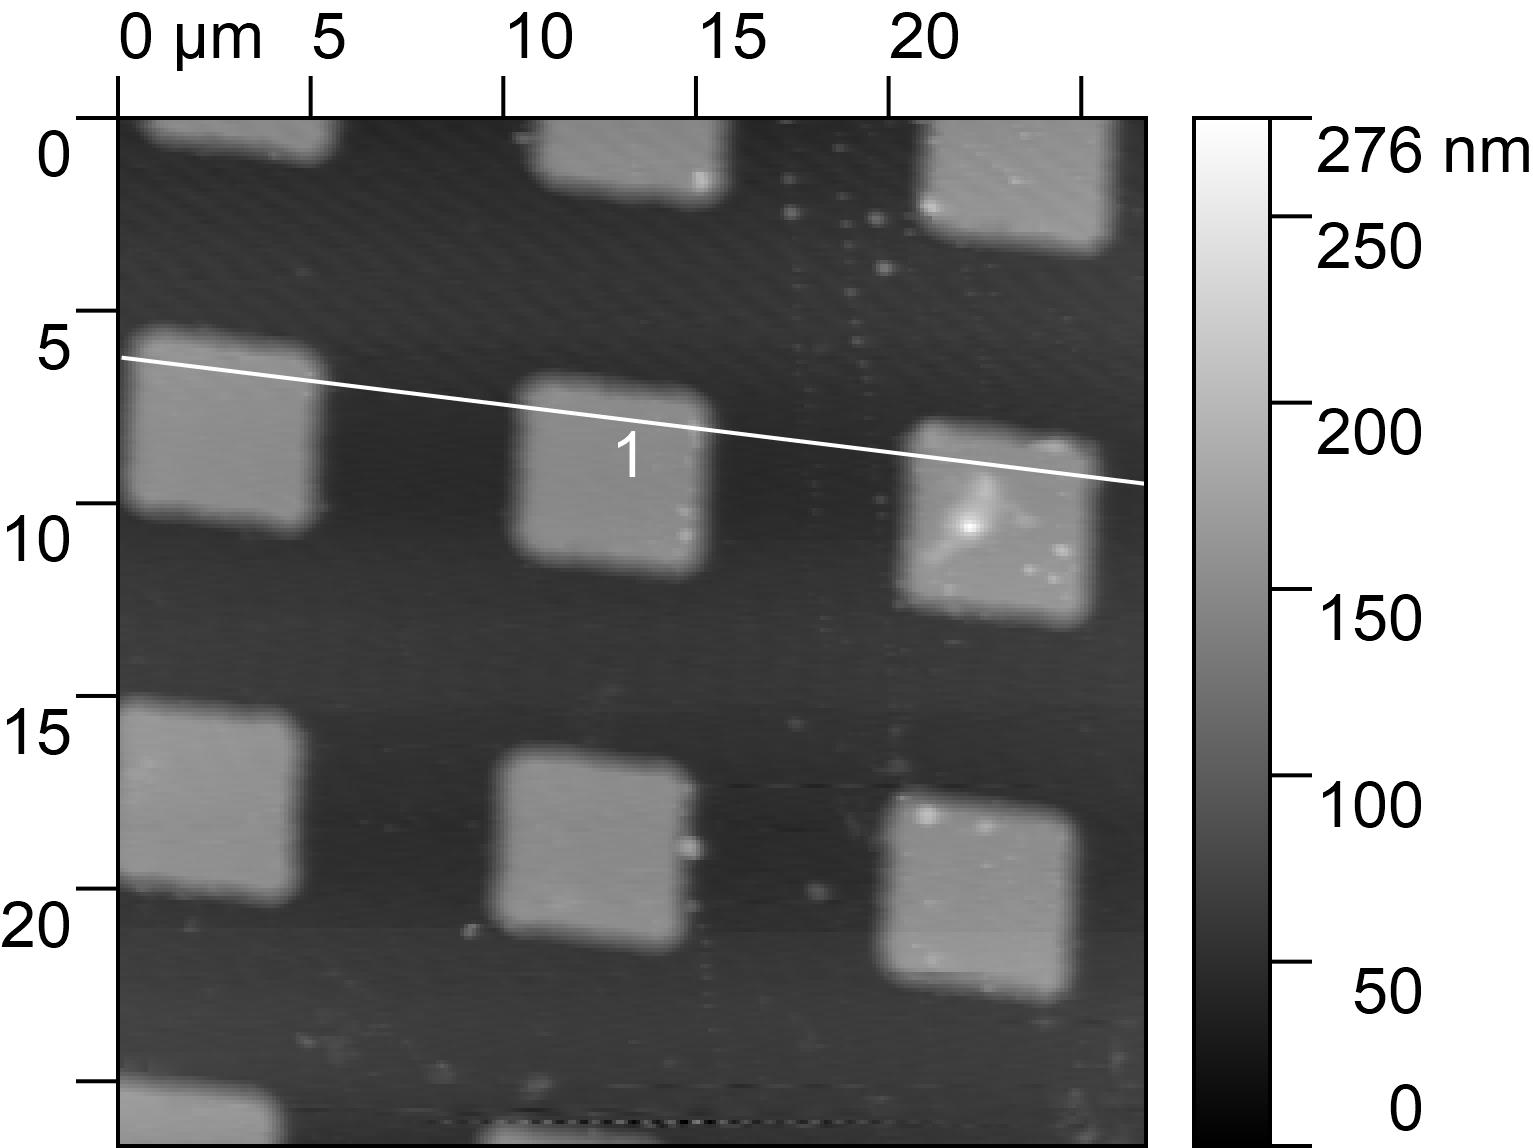
\includegraphics[width=.49\linewidth]{images/Kali/Top}}
			\subcaptionbox{3D-Sicht \label{fig_kali_3d}}{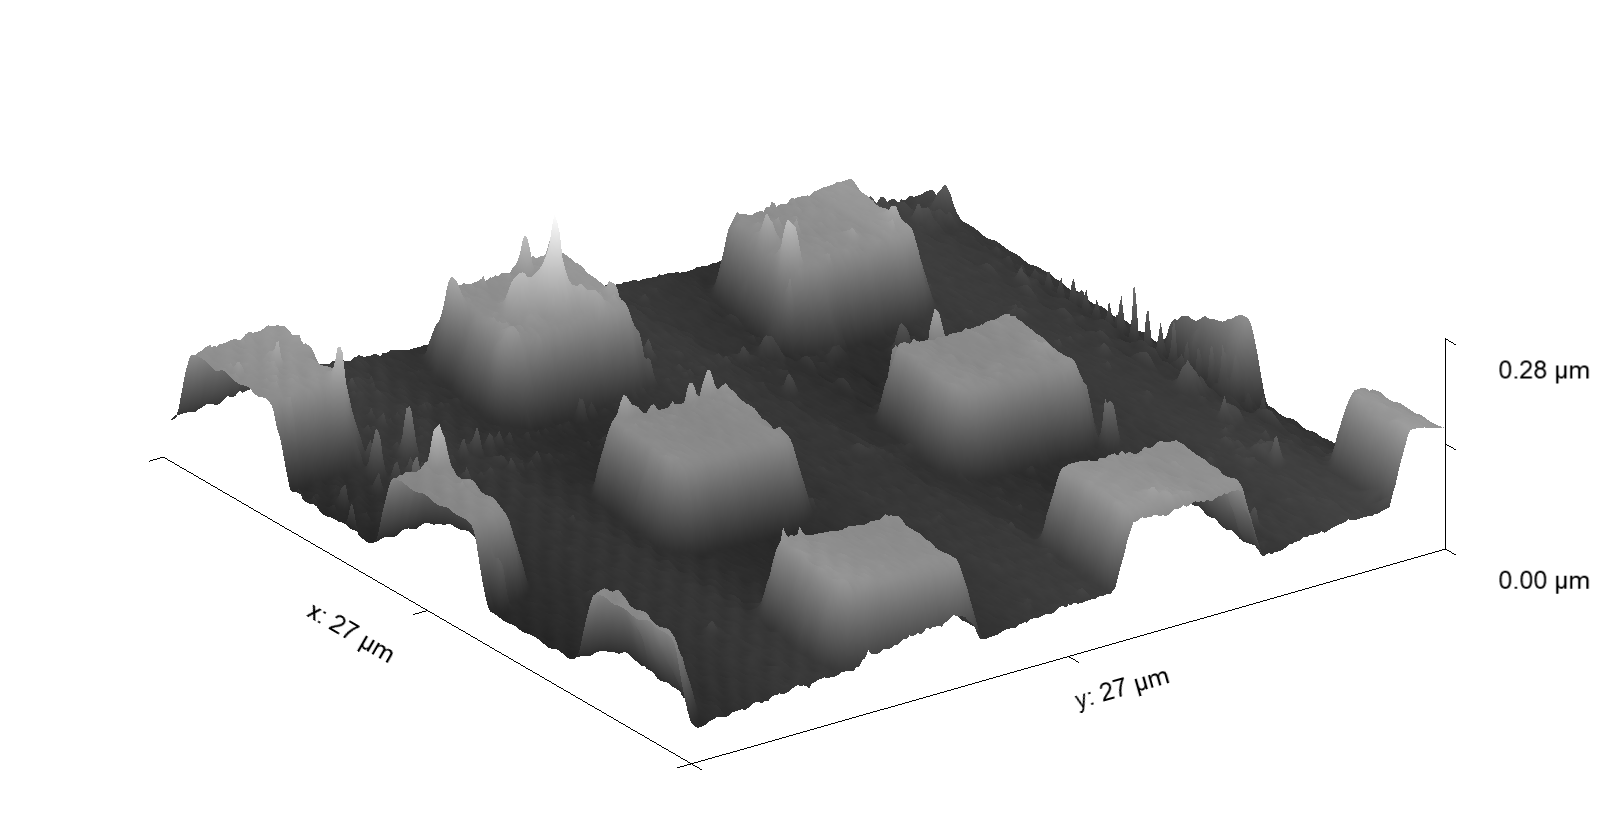
\includegraphics[width=.49\linewidth]{images/Kali/3D}}
			\subcaptionbox{Profil 1 \label{fig_kali_profil}}{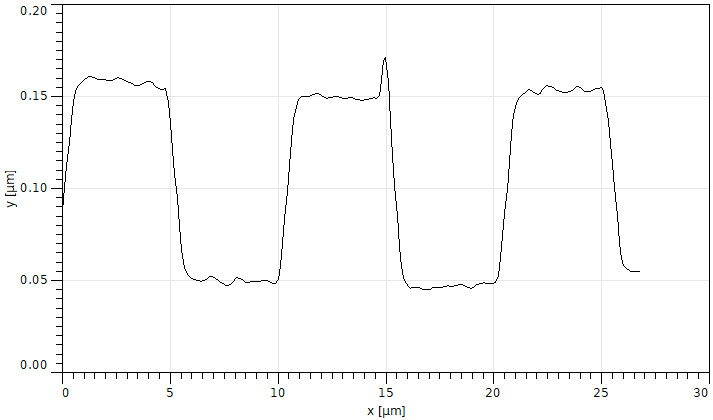
\includegraphics[width=.7\linewidth]{images/Kali/Profil}}
			\caption{Kalibrierungsprobe.}
\end{figure}


\subsubsection{Datenträgerproben}
%TODO 1x Pit nach unten 2x nach oben
\begin{figure}[H]
			\subcaptionbox{Draufsicht \label{fig_dvd_top}}{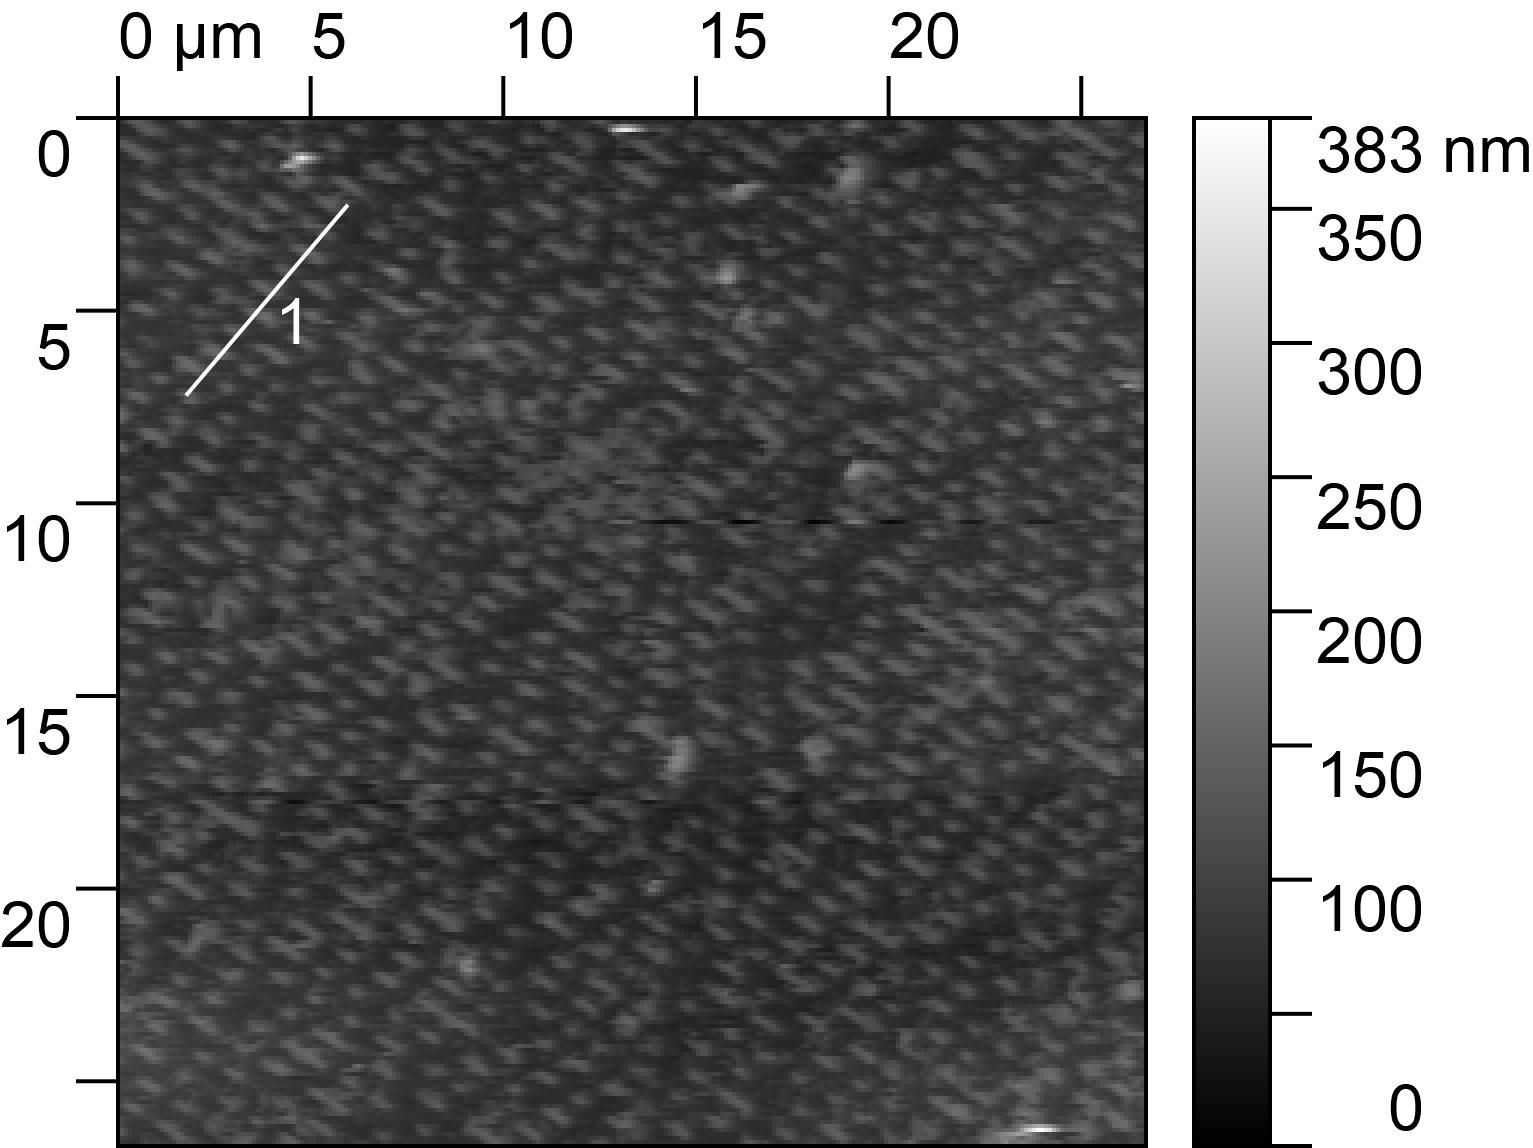
\includegraphics[width=.49\linewidth]{images/DVD/Top}}
			\subcaptionbox{3D-Sicht \label{fig_dvd_3d}}{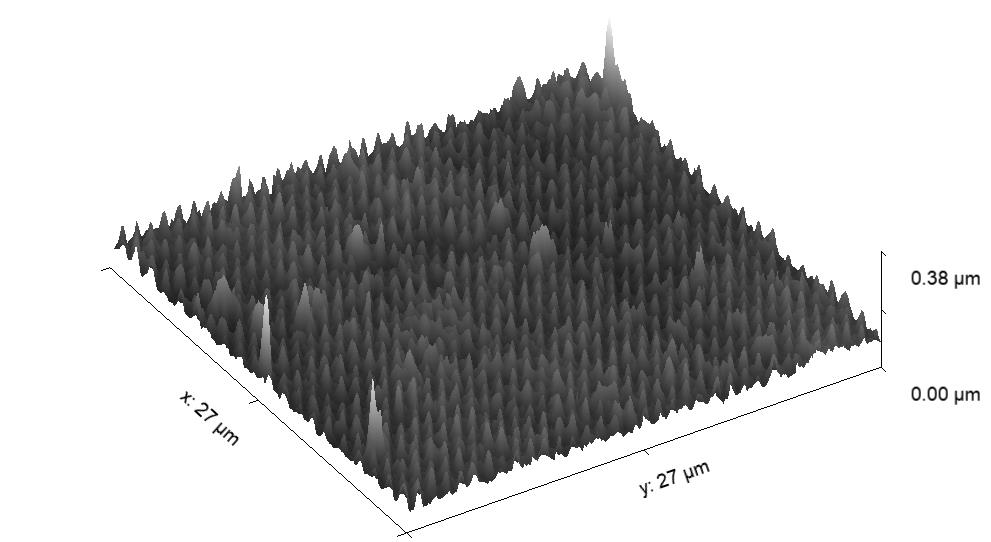
\includegraphics[width=.49\linewidth]{images/DVD/3D}}
			\subcaptionbox{Vergrößerte Draufsicht \label{fig_dvd_top_zoom}}{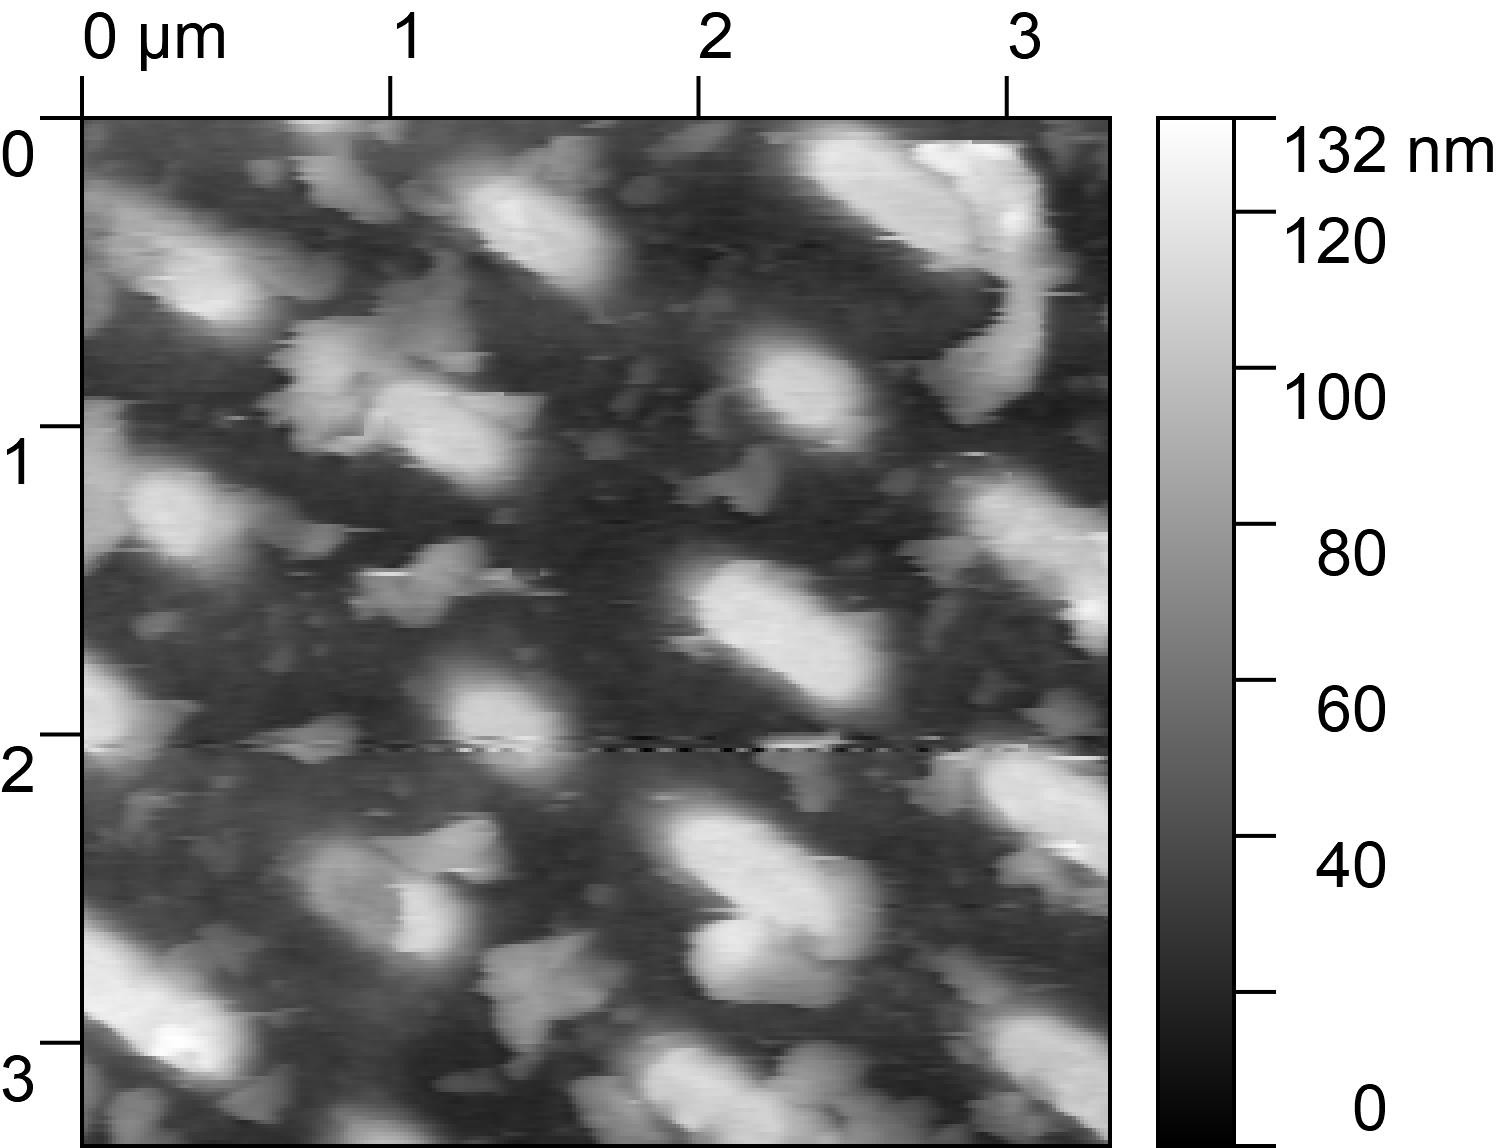
\includegraphics[width=.49\linewidth]{images/DVD/Top_zoom}}
			\subcaptionbox{Vergrößerte 3D-Sicht \label{fig_dvd_3d_zoom}}{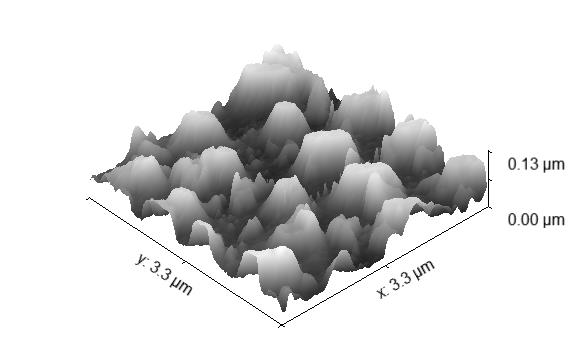
\includegraphics[width=.49\linewidth]{images/DVD/3D_zoom}}
			\subcaptionbox{Profil 1.  Der gemessene Abstand beträgt \SI{5.48}{\mu m}.
			 \label{fig_dvd_profil}}{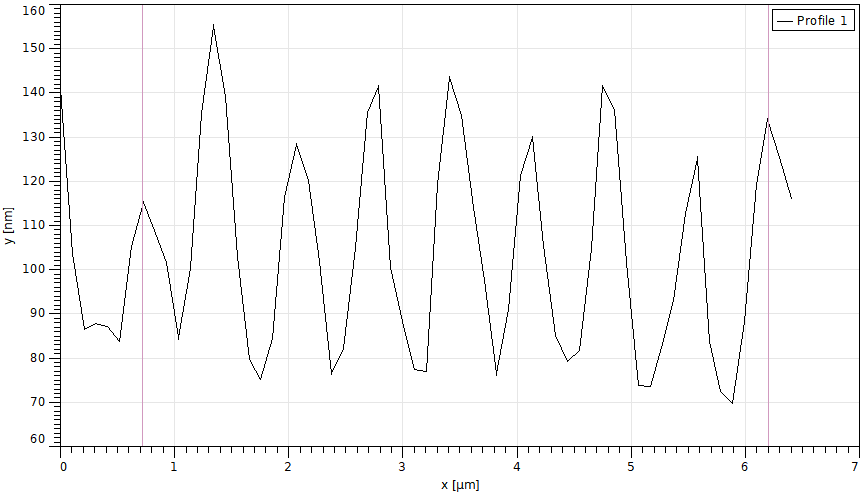
\includegraphics[width=.7\linewidth]{images/DVD/Profil}}
			\caption{Probe 1.}
\end{figure}


\begin{figure}[H]
			\subcaptionbox{Draufsicht \label{fig_cd_top}}{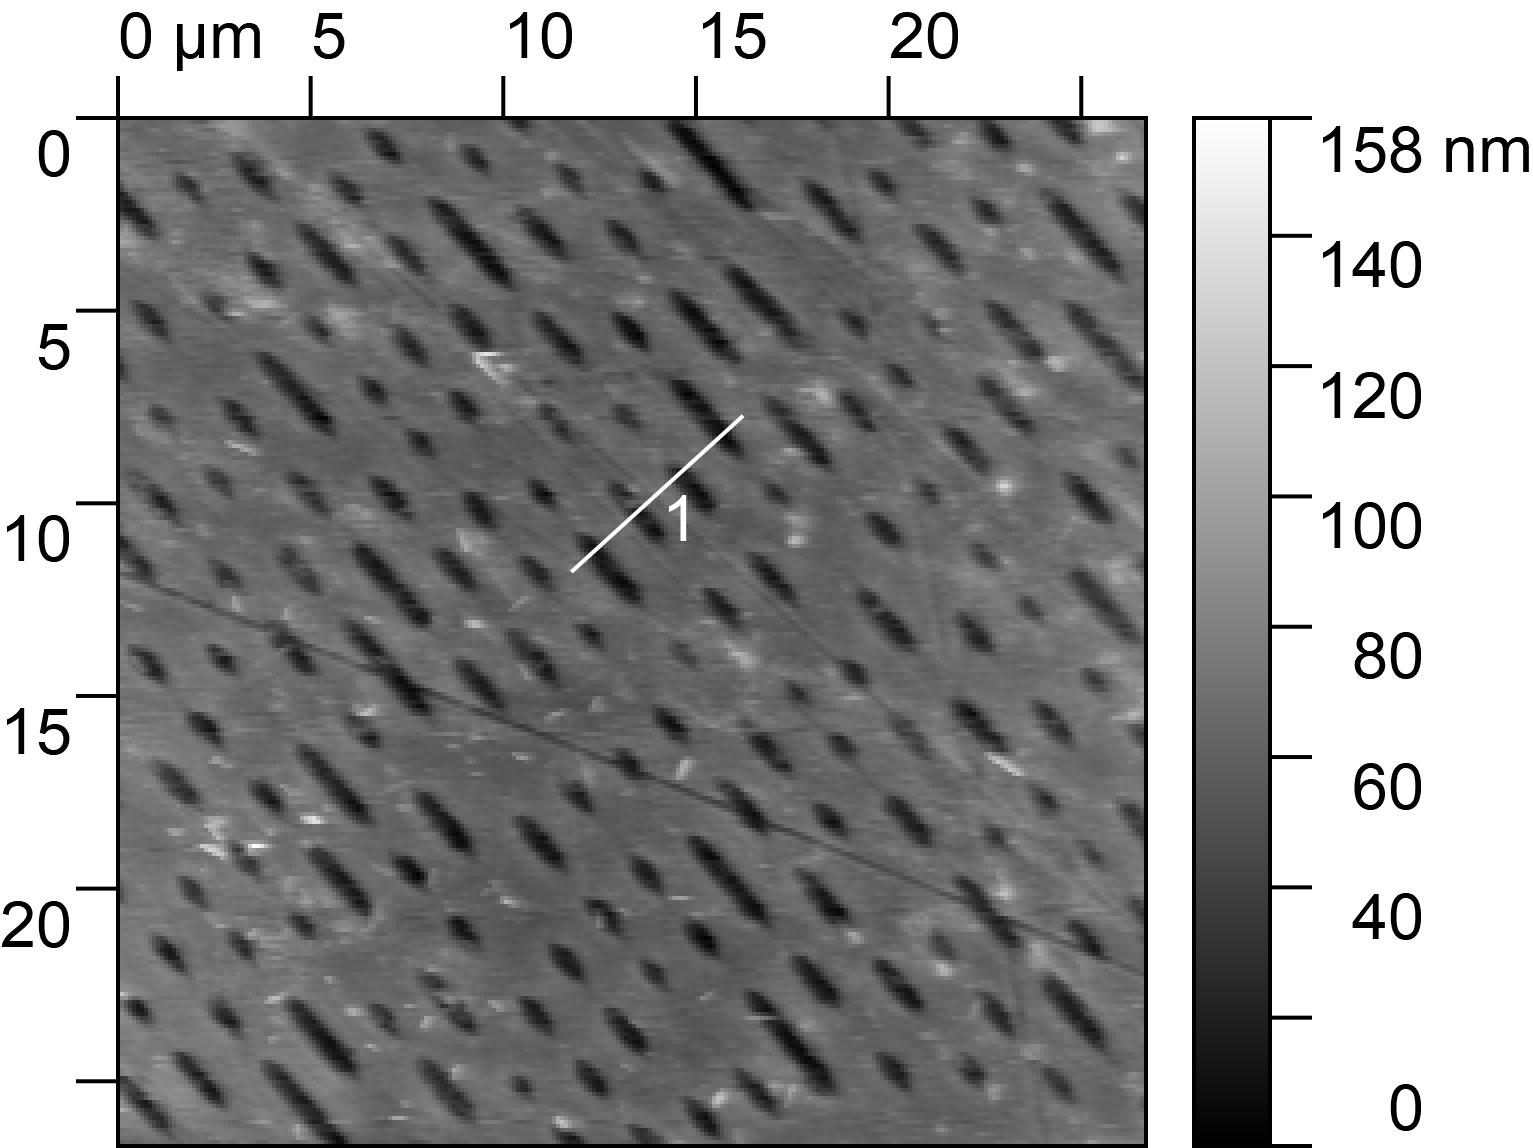
\includegraphics[width=.49\linewidth]{images/CD/Top}}
			\subcaptionbox{3D-Sicht \label{fig_cd_3d}}{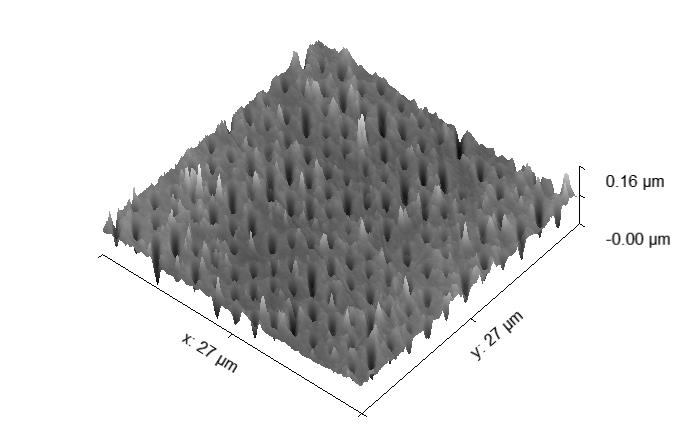
\includegraphics[width=.49\linewidth]{images/CD/3D}}
			\subcaptionbox{Vergrößerte Draufsicht \label{fig_cd_top_zoom}}{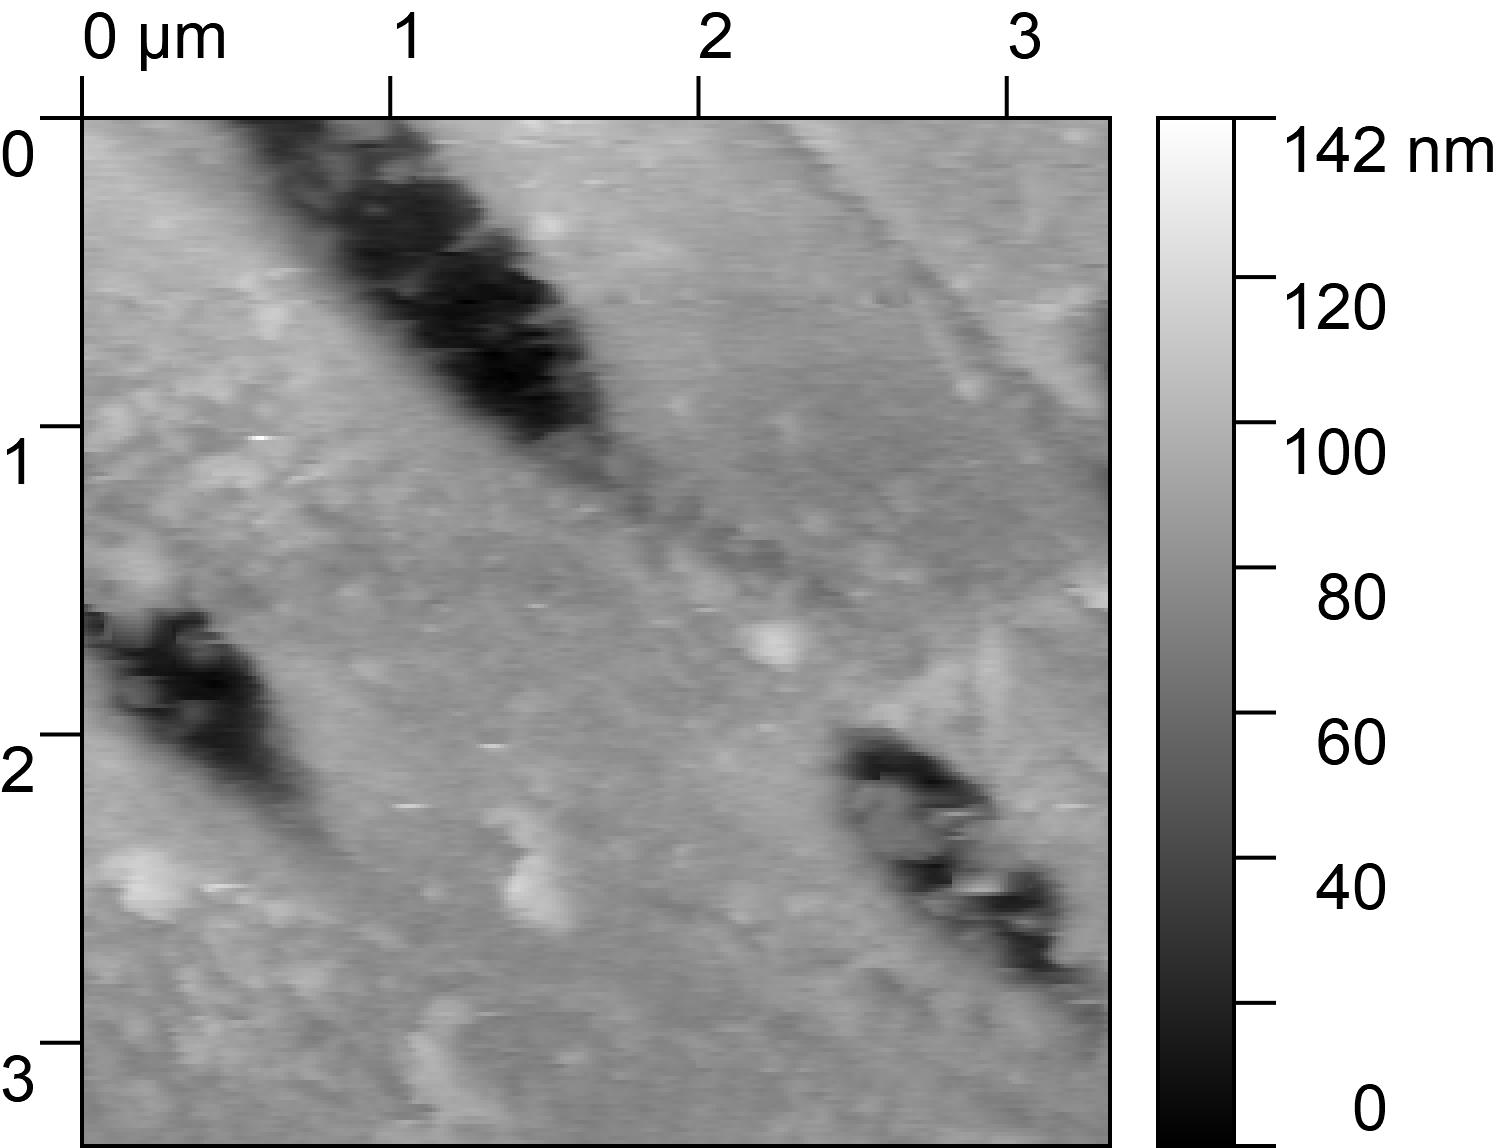
\includegraphics[width=.49\linewidth]{images/CD/Top_zoom}}
			\subcaptionbox{Vergrößerte 3D-Sicht \label{fig_cd_3d_zoom}}{\includegraphics[width=.49\linewidth]{images/CD/3D_zoom}}
			\subcaptionbox{Profil 1. Der gemessene Abstand beträgt \SI{4.535}{\mu m}. % Die Tiefe des Minimums bei $x\approx\SI{5.3}{\mu m}$ beträgt \SI{58.5}{nm}.
			 \label{fig_cd_profil}}{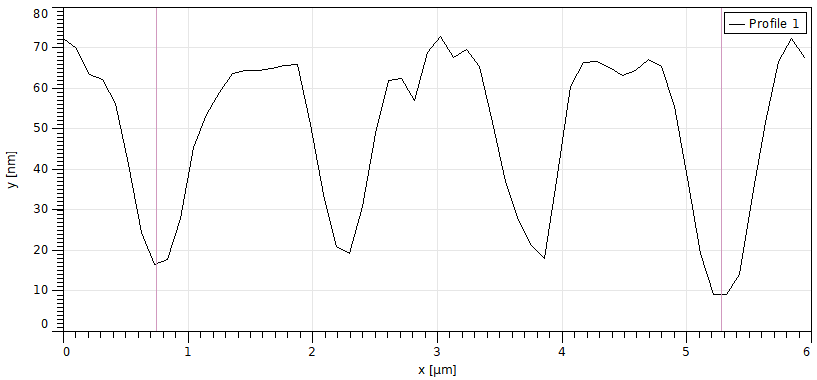
\includegraphics[width=.7\linewidth]{images/CD/Profil}}
			\caption{Probe 2.}
\end{figure}

\begin{figure}[H]
			\subcaptionbox{Draufsicht \label{fig_br_top}}{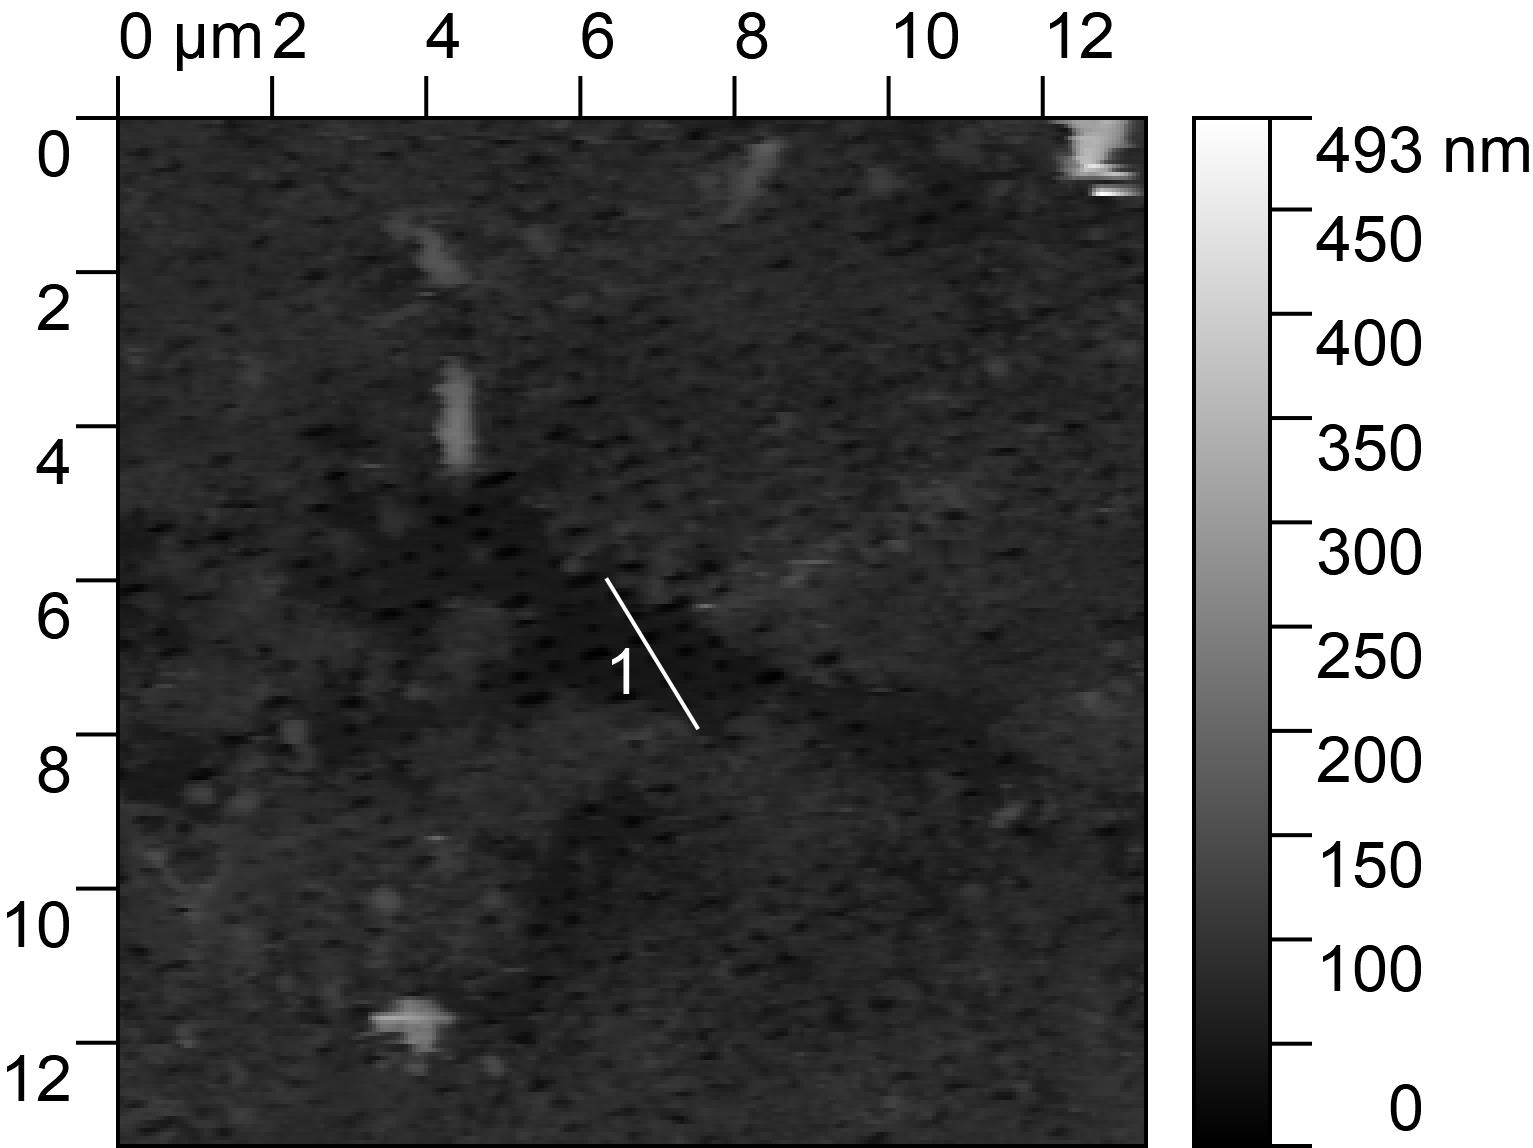
\includegraphics[width=.49\linewidth]{images/BR/Top}}
			\subcaptionbox{3D-Sicht \label{fig_br_3d}}{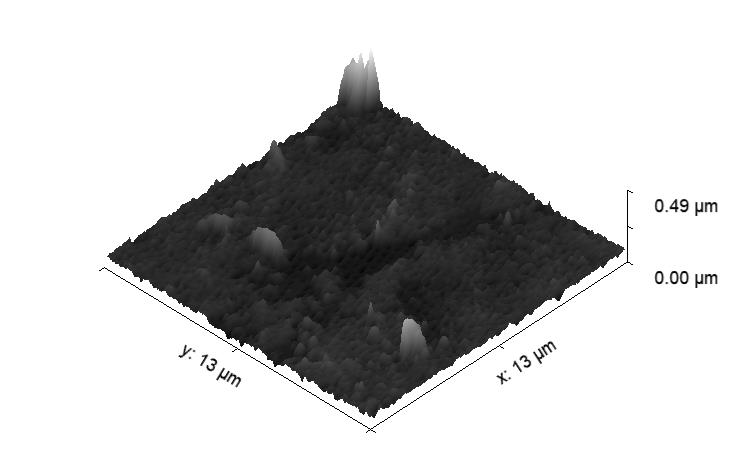
\includegraphics[width=.49\linewidth]{images/BR/3D}}
			\subcaptionbox{Vergrößerte Draufsicht \label{fig_br_top_zoom}}{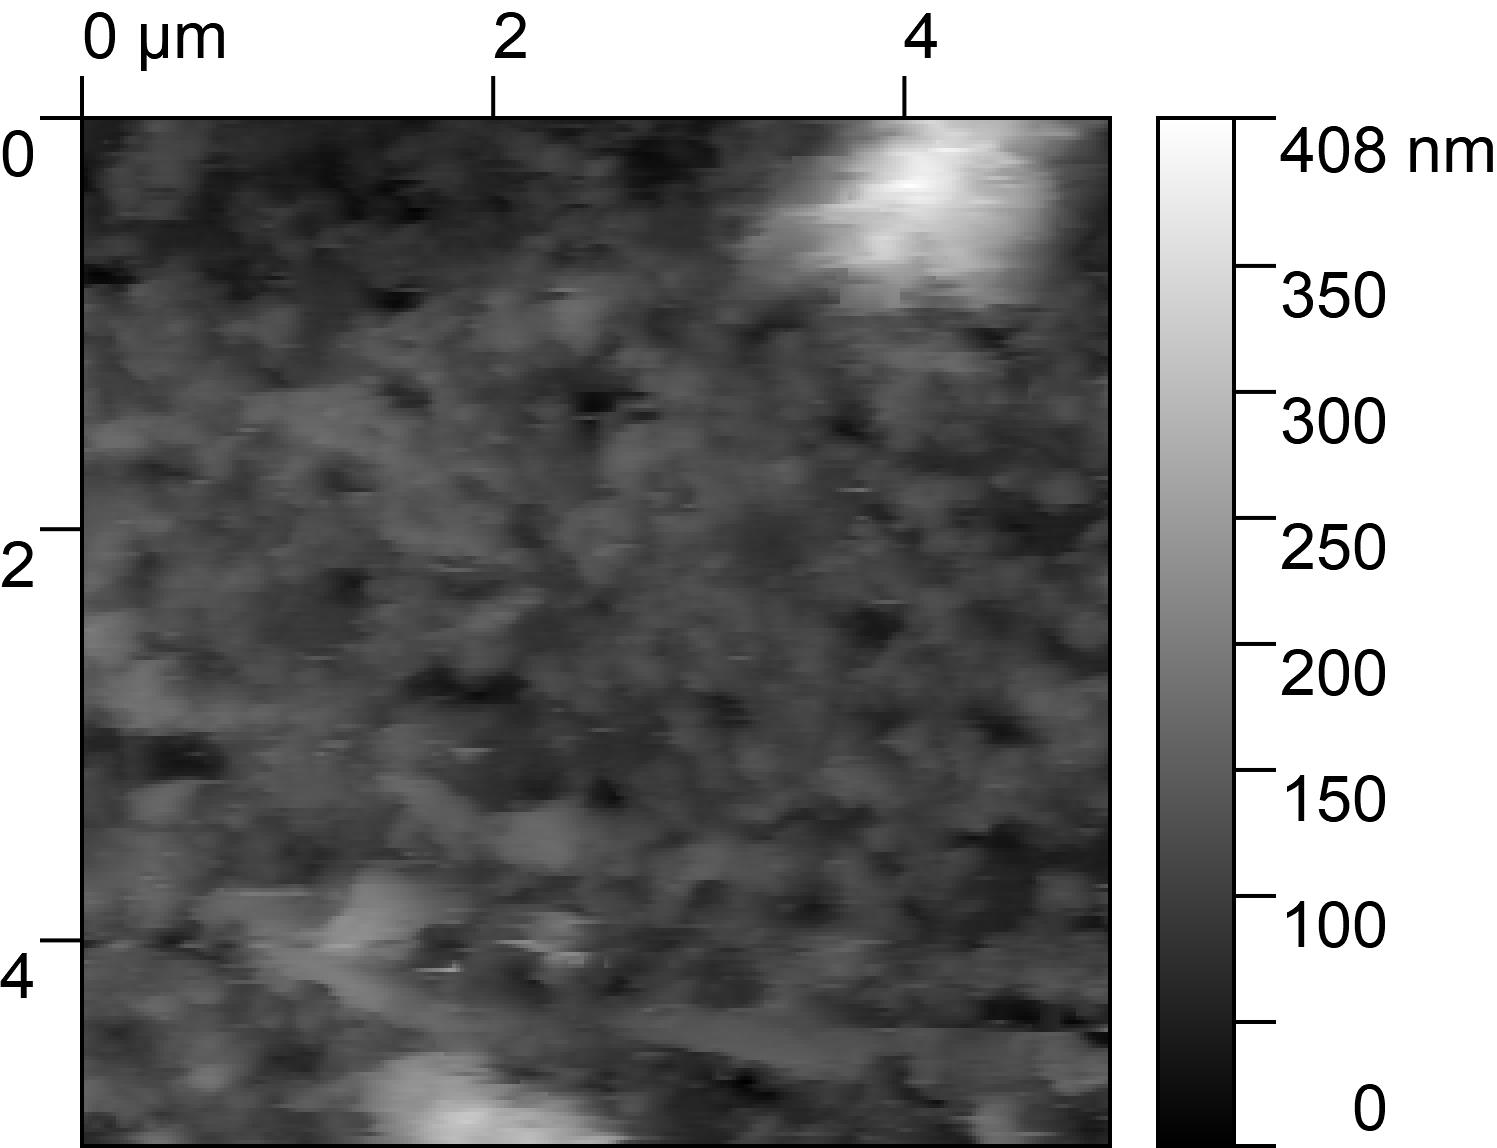
\includegraphics[width=.49\linewidth]{images/BR/Top_zoom}}
			\subcaptionbox{Vergrößerte 3D-Sicht \label{fig_br_3d_zoom}}{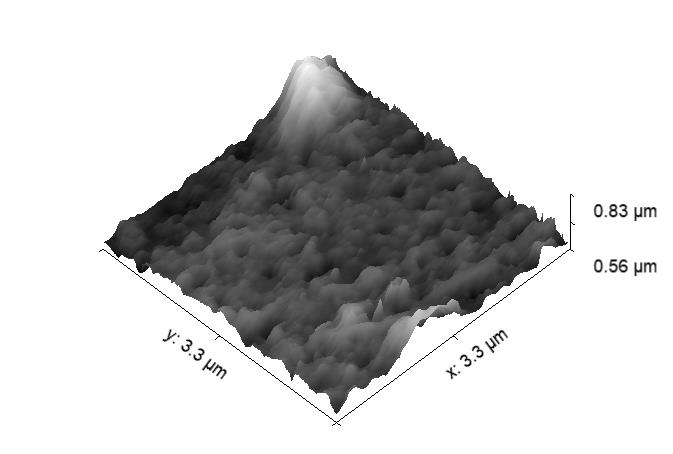
\includegraphics[width=.49\linewidth]{images/BR/3D_zoom}}
			\subcaptionbox{Profil 1. Der gemessene Abstand zwischen den zwei Horizontalen beträgt \SI{1.64}{\mu m}. %Die Tiefe des Minimums bei $x\approx\SI{1}{\mu m}$ beträgt \SI{39.3}{nm}.
			\label{fig_br_profil}}{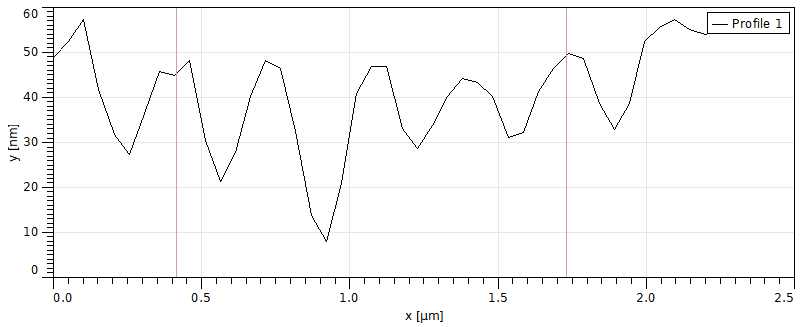
\includegraphics[width=.7\linewidth]{images/BR/Profil}}
			\caption{Probe 3.}
\end{figure}

\subsubsection{TGT1-Probe}

%TODO dynamische Modus
%TODO optimiert sodass minimal unschön

\begin{figure}[H]
			\subcaptionbox{Draufsicht
			 \label{fig_tgt_top}}{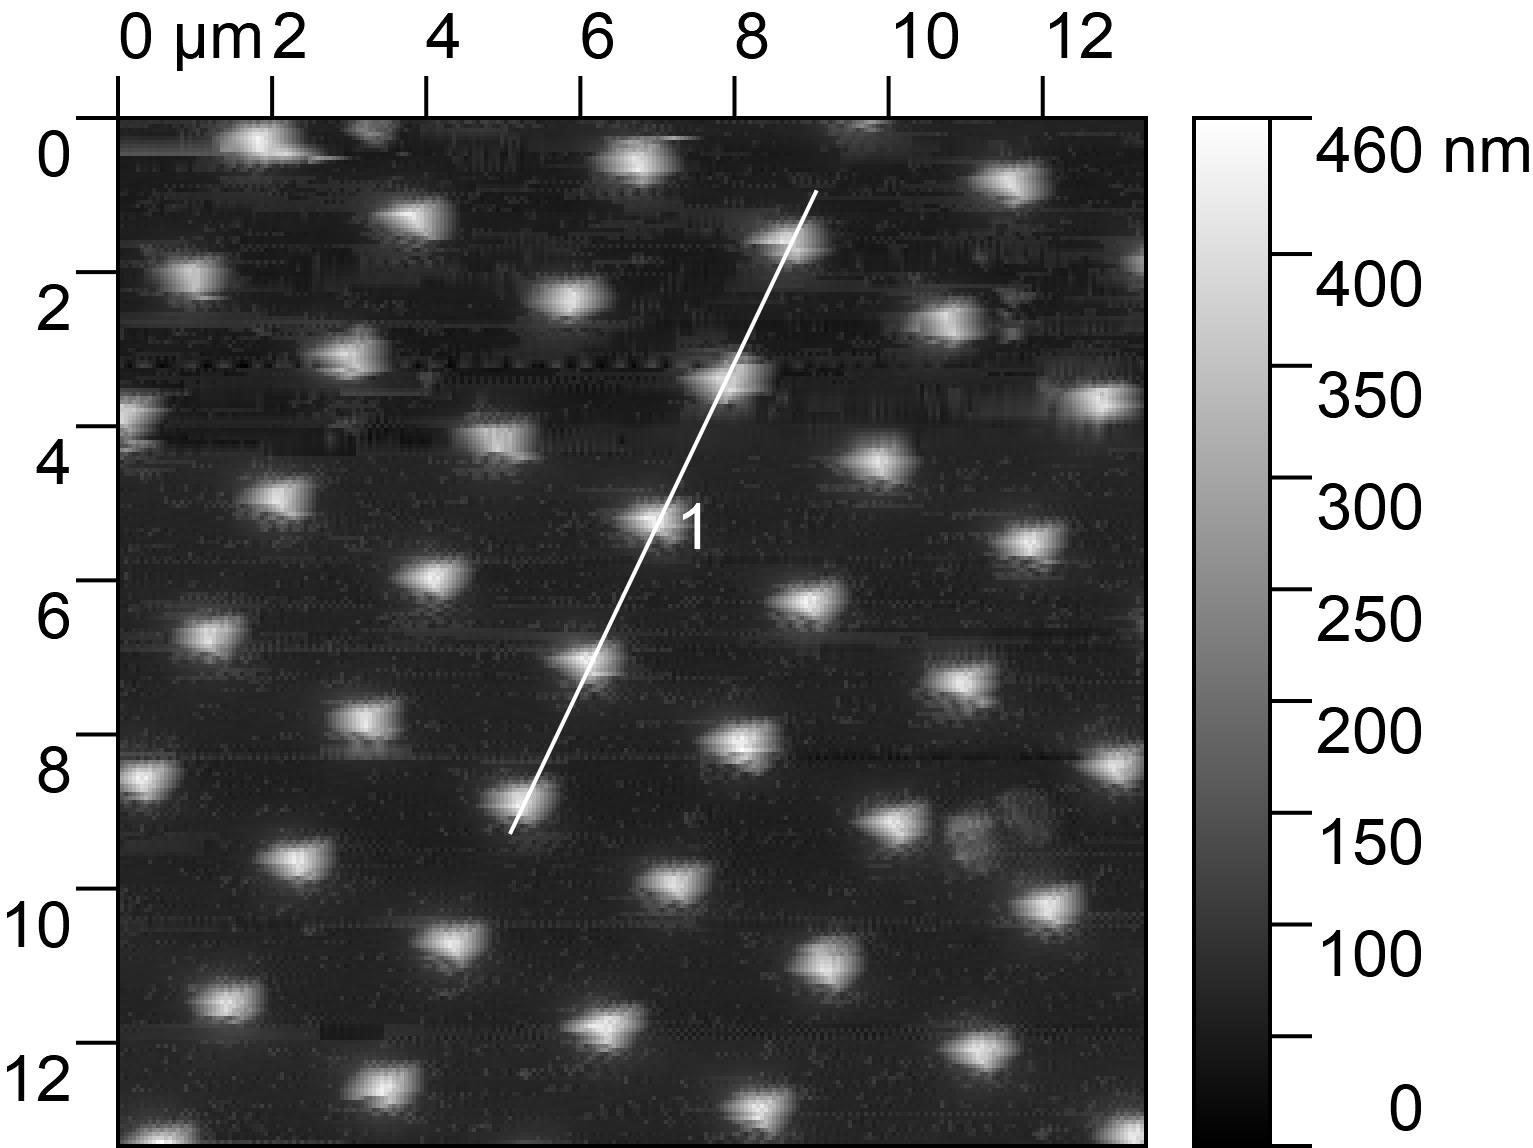
\includegraphics[width=.49\linewidth]{images/TGT/Top}}
			\subcaptionbox{3D-Sicht
			\label{fig_tgt_3d}}{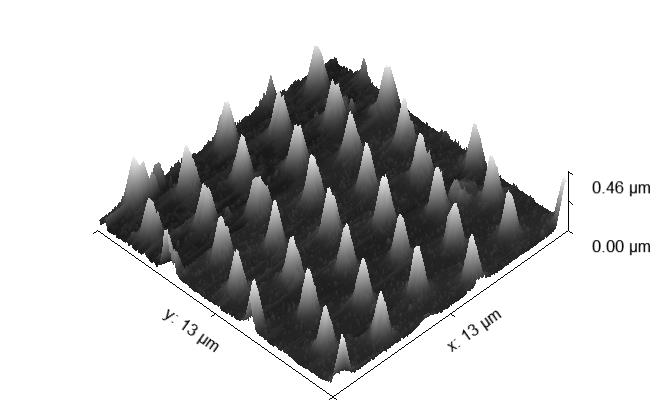
\includegraphics[width=.49\linewidth]{images/TGT/3D}}
			\subcaptionbox{Profil 1
			\label{fig_tgt_profil}}{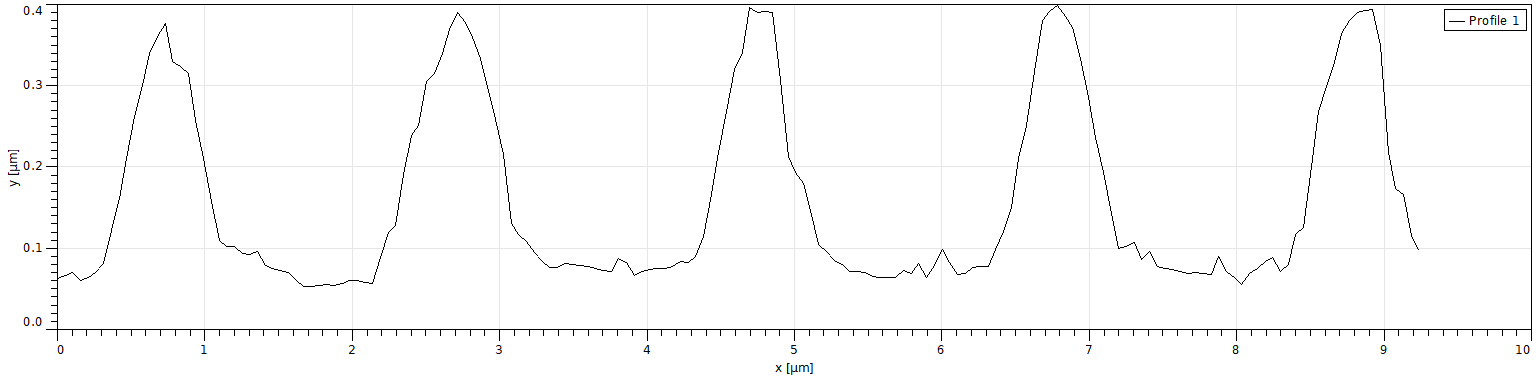
\includegraphics[width=.99\linewidth]{images/TGT/Profil}}
			\caption{TGT1 Probe.}
\end{figure}

\begin{figure}[H]
			\subcaptionbox{Draufsicht
			 \label{fig_tgt_top_zoom}}{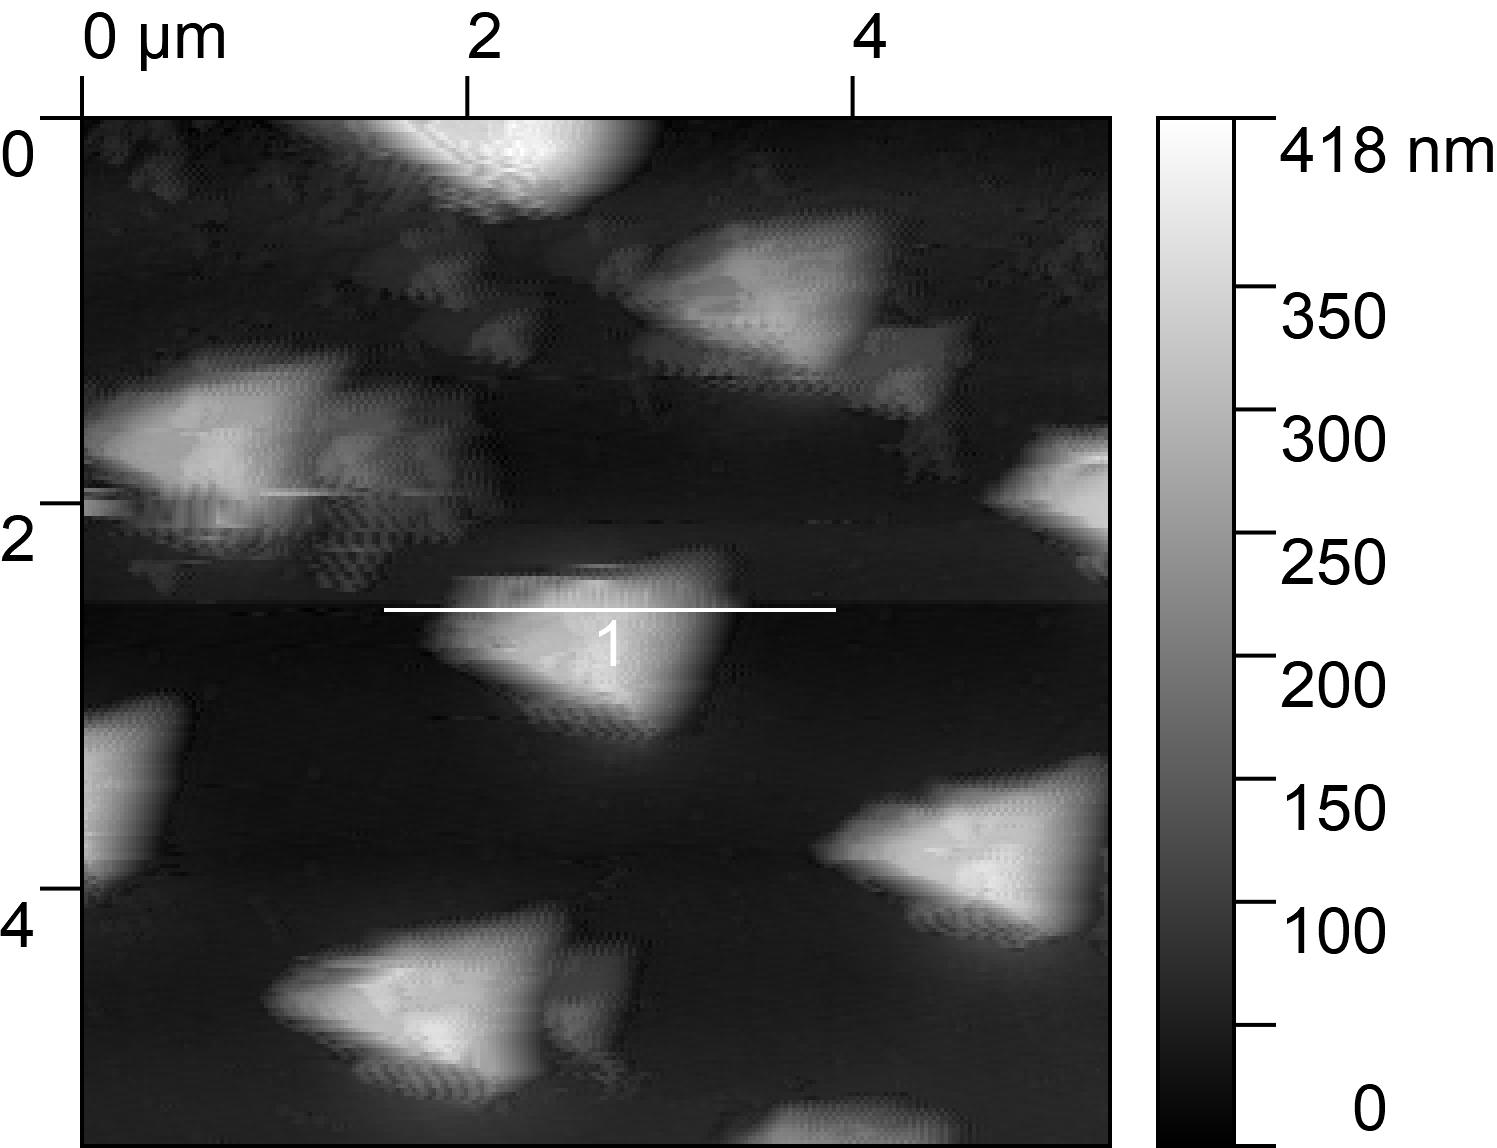
\includegraphics[width=.49\linewidth]{images/TGT/Top_zoom}}
			\subcaptionbox{3D-Sicht
			\label{fig_tgt_3d_zoom}}{\includegraphics[width=.49\linewidth]{images/TGT/3D_zoom}}
			\subcaptionbox{Profil 1. Fit ist ein Kreis mit dem Radius $r= \SI{1.204 +-0.016}{\mu m}$
			\label{fig_tgt_profil_zoom}}{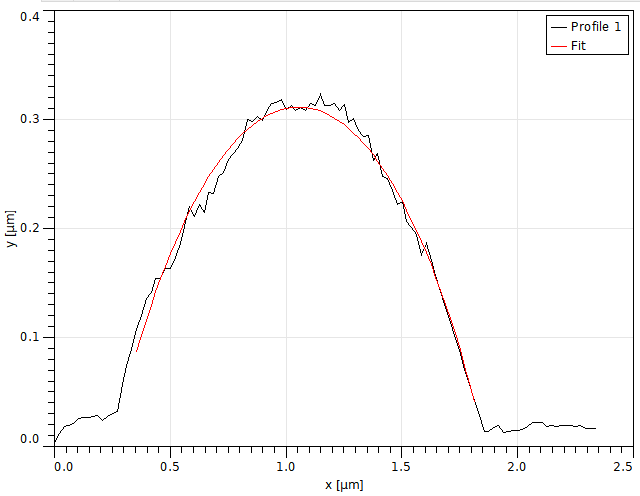
\includegraphics[width=.6\linewidth]{images/TGT/Profil_zoom}}
			\caption{TGT1 Probe.}
\end{figure}

	\subsubsection{Unsicherheiten} %TODO GGF IN DATENANYLSY
	Folgende Unsichheiten waren auf den Behältern der Cantilevers für die Federkonstante $c$ angegeben:
	\begin{description}
		\item[statischer Modus:] \SI{0.02}{N/m} - \SI{0.77}{N/m} % 0.395+-0.375
		\item[dynamischer Modus:] \SI{21}{N/m} - \SI{98}{N/m}
	\end{description}
	Alle weiteren Unsicherheiten verschwinden gegenüber der Unsichheit der Federkonstante.
	\subsection{Datenanalyse}
	%TODO Berechung nach Aufgabenstellung
	\subsubsection{Kalibrierungsprobe} \label{sss_kali}
	% snap-offs 26.287, 28, 25.557, 35.1, 29.6 => 28.9
	Die Adhäsionskräft, welche an einem Punkt auf den Cantilever wirkt, während dieser sich von dem Material wegbewegt, lässt sich direkt aus dem Snap-off s und der Federkonstante bestimmen:
	\begin{equation}
			\label{eq_adh}
			F_\text{adh} = s \cdot c
	\end{equation}
	Es folgt $F_\text{adh}=\SI{11.4+-10.8}{nN}$, wobei über die fünf gemessenen Hysteresen (\crefrange{fig_kali_ds1}{fig_kali_ds5}) gemittelt wird.

	\subsubsection{Datenträgerproben} %CD/DVD/BR}
	Analog zu \cref{sss_kali} lassen sich aus den Kraft-Abstand-Spektroskopie Kurven (\cref{fig_dvd_ds},\cref{fig_cd_ds} und \cref{fig_br_ds}) die Adhäsionskräfte der Datenträger bestimmen.
	Die resultierenden Adhäsionskräfte sind in \cref{tb_adh} aufgeführt.

\begin{table}[H]
		\centering
		\begin{tabular}{ c | c | c | c }
			 & Probe 1 & Probe 2 & Probe 3\\ \hline
			$F_\text{adh}$ & \SI{17.6+-16.7}{nN} & \SI{20.0+-19.0}{nN} &\SI{14.0+-13.3}{nN} \\
		\end{tabular}
		\caption{Adhäsionskräfte die auf die Spitze des Cantilevers wirken bei Kraft-Abstand-Spektroskopie.}
		\label{tb_adh}
\end{table}

	Die Spurbreite $b_\text{Spur}$ des jeweiligen Datenträgers ergibt sich gemittelt aus den in \cref{fig_dvd_profil},\cref{fig_cd_profil} bzw. \cref{fig_br_profil} gemessenen Abständen mehrer Spuren.
	Der Abstand wird trivialerweise durch die Anzahl der Spuren dividiert.
	Es folgen die Spurbreiten in \cref{tb_spur}.
	Analog lassen sich Pit-Länge $l_\text{Pit}$ , Pit-Breite $b_\text{Pit}$ und Pit-Tiefe $t_\text{Pit}$ bestimmen.
	Diese sind ebenfalls in \cref{tb_spur} aufgeführt.

\begin{table}[H]
		\centering
		\begin{tabular}{ c | c | c | c }
			 & Probe 1 & Probe 2 & Probe 3\\ \hline
			$b_\text{Spur}$ & \SI{690}{nm} & \SI{1510}{nm} &\SI{330}{nm} \\
			$l_\text{Pit}$ & \SI{530}{nm} & \SI{873}{nm} &\SI{170}{nm} \\
			$b_\text{Pit}$ & \SI{390}{nm} & \SI{682}{nm} &\SI{321}{nm} \\
			$t_\text{Pit}$ & \SI{63}{nm} & \SI{48}{nm} &\SI{41}{nm} \\
		\end{tabular}
		\caption{Spurbreite $b_\text{Spur}$, Pit-Länge $l_\text{Pit}$, Pit-Breite $b_\text{Pit}$, Pit-Tiefe $t_\text{Pit}$ der jeweiligen Datenträger 1-3.
		Die Unsicherheiten sind mit \SI{5}{\%} abgeschätzt.}
		\label{tb_spur}
	\end{table}

	% 1) DVD
	% 2) CD
	% 3) BR
	\subsubsection{TGT1 Probe} %TODO Name
	Aus dem Profil einer gemessenen Spitze \cref{fig_tgt_profil_zoom} lässt sich mittels einer Anpassung an einen Kreis der Radius der Spitze des Cantilevers bestimmen.
	Es ergibt sich ein Radius $r=\SI{1.204 +-0.016}{\mu m}$.

	\subsection{Diskussion}
	%TODO Bezug/Nutzen oder sonst was
	%TODO auch hier die Hypothese wiederholen
	%TODO keine Messwerte hier, nach manchen Menschen, zumindest "direkt" erstellte Diagramme net hier, auch wenn Lesbarkeit-bla

 %TODO vegleich literatur Box+ Nanosurf spitzen radius
 %TODO neuer => weniger adhäsion??
 %TODO DVD am tiefsten/höchsten ?? ggf weil des des einzige andersrum ist.
\begin{table}[H]
	%TODO tabelle für zusammen vergleichen der Adhäsionskräfte?
		\centering
		\begin{tabular}{ c | c }
			 & Kalibrierungsprobe\\ \hline
			$F_\text{adh}$ & \SI{10.8+-11.4}{nN} \\
		\end{tabular}
		\caption{Adhäsionskräfte die auf die Spitze des Cantilevers wirken bei Kraft-Abstand-Spektroskopie.} %TODO mehr
		\label{tb_ds}
	\end{table}

	%TODO CD/DVD https://www.nickles.de/c/s/Klein-rund-und-duenn-was-steckt-in-der-DVD-267-1.html sonst findet man auch mit spurbreite googlei für BR
	%TODO Alles bsichen zu klein => Skalierung nicht optimal

	\section{Schlussfolgerung}
	%TODO Rückgriff auf Hypothese und drittes Nennen dieser

	%TODO Quellen zitieren, Websiten mit Zugriffsdatum
	%TODO Verweise auf das Laborbuch (sind erlaubt)
	%TODO Tabelle + Bilder mit Beschriftung
	%\printbibliography
	\section{Anhang}

\begin{figure}[H]
			\centering
			\subcaptionbox{snap-off $s=\SI{29.6}{nm}$ \label{fig_kali_ds1}}{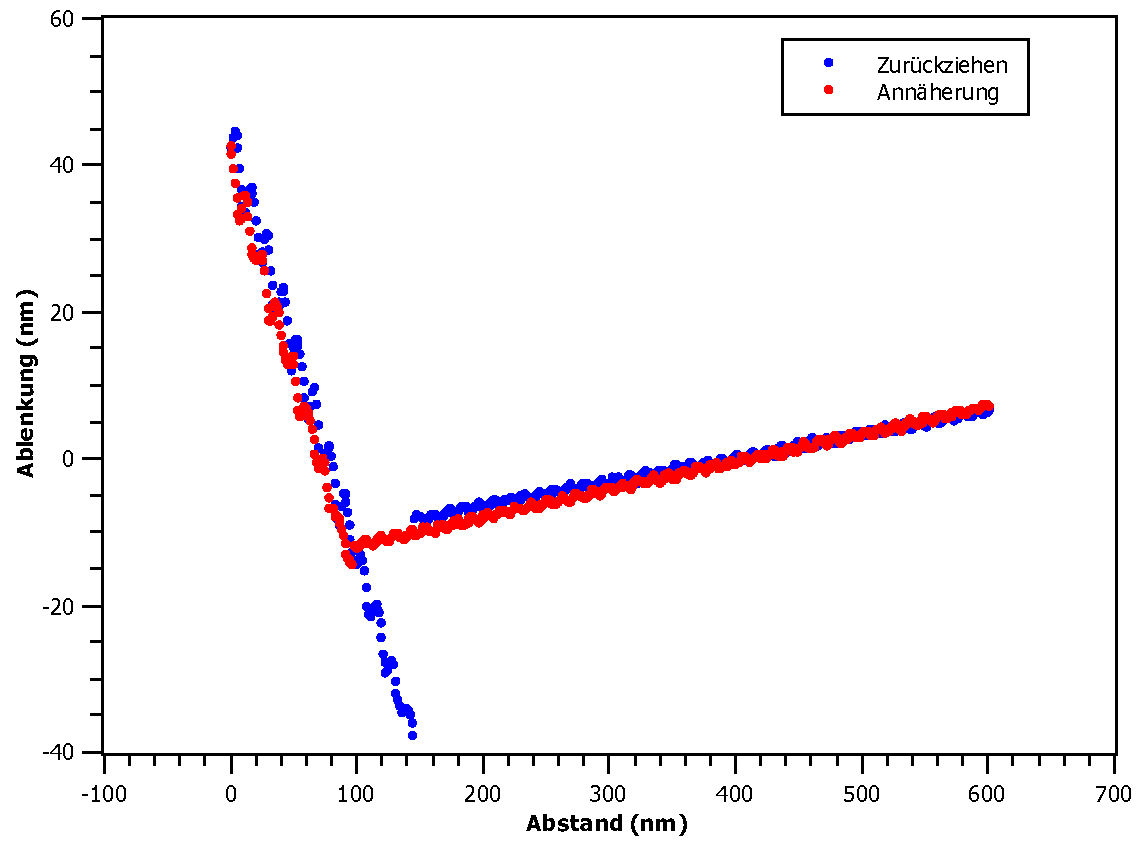
\includegraphics[width=.49\linewidth]{images/Kali/DS1}}
			\subcaptionbox{snap-off $s=\SI{35.1}{nm}$  \label{fig_kali_ds2}}{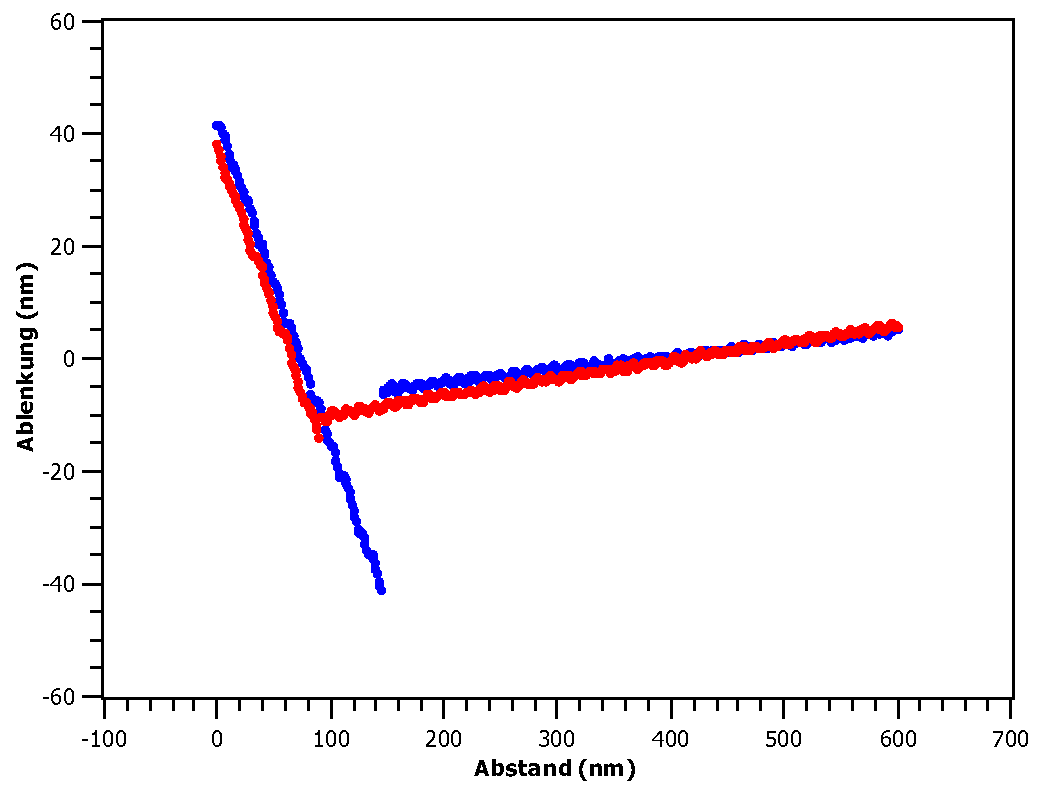
\includegraphics[width=.49\linewidth]{images/Kali/DS2}}
			\subcaptionbox{snap-off $s=\SI{25.6}{nm}$  \label{fig_kali_ds3}}{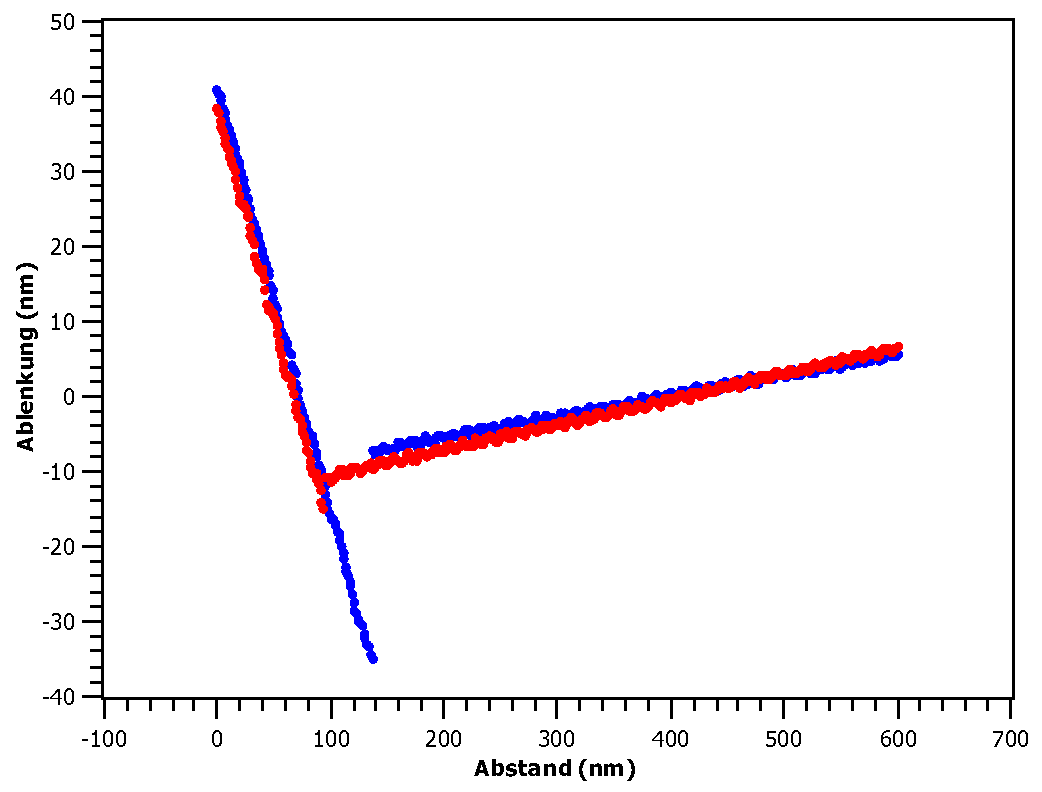
\includegraphics[width=.49\linewidth]{images/Kali/DS3}}
			\subcaptionbox{snap-off $s=\SI{26.3}{nm}$  \label{fig_kali_ds4}}{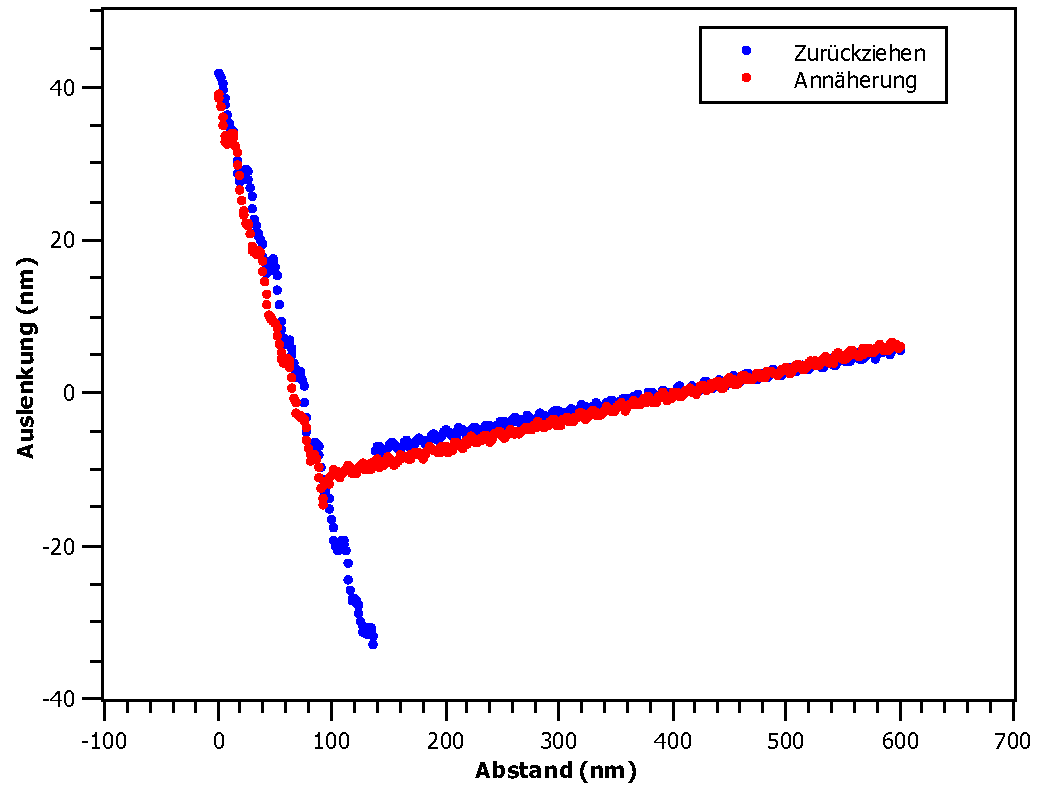
\includegraphics[width=.49\linewidth]{images/Kali/DS4}}
			\subcaptionbox{snap-off $s=\SI{28.0}{nm}$
			\label{fig_kali_ds5}}{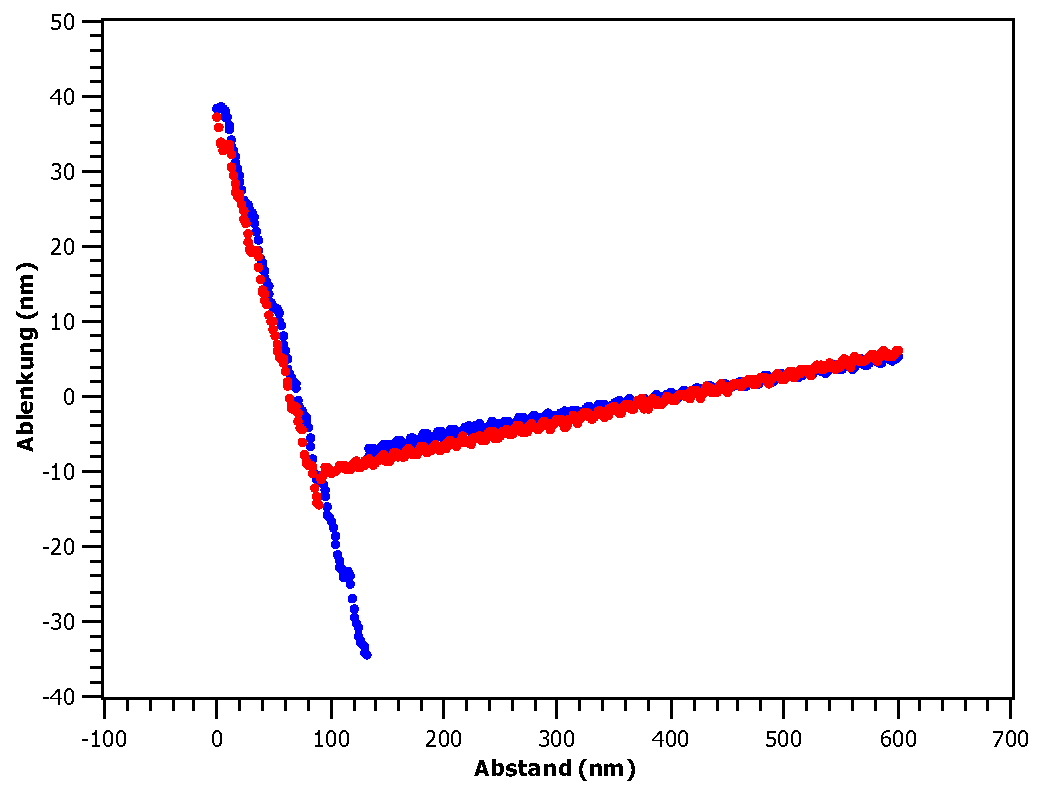
\includegraphics[width=.49\linewidth]{images/Kali/DS5}}
			\caption{Kraft-Abstands-Spektroskopie der Kalibrierungsprobe. Gemittelter snap-off $s=\SI{24.1}{nm}$.}
\end{figure}

\begin{figure}[H]
			\centering
			\subcaptionbox{snap-off $s=\SI{46.2}{nm}$  \label{fig_dvd_ds1}}{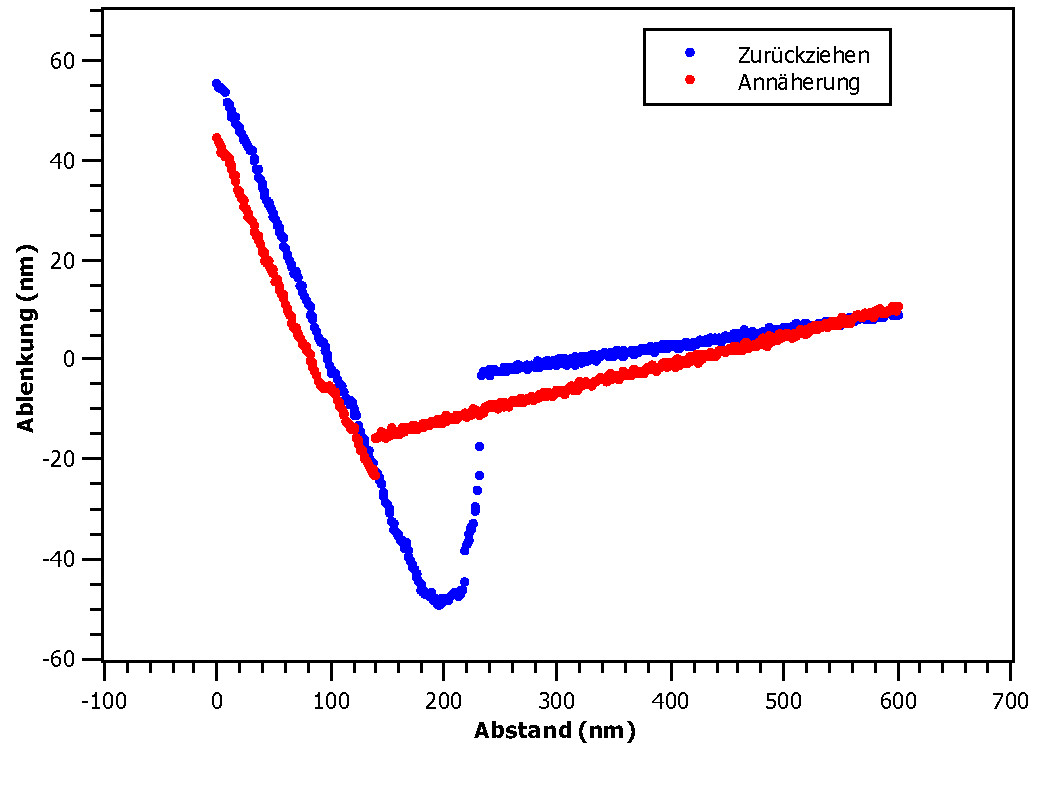
\includegraphics[width=.49\linewidth]{images/DVD/DS1}}
			\subcaptionbox{snap-off $s=\SI{50.0}{nm}$  \label{fig_dvd_ds2}}{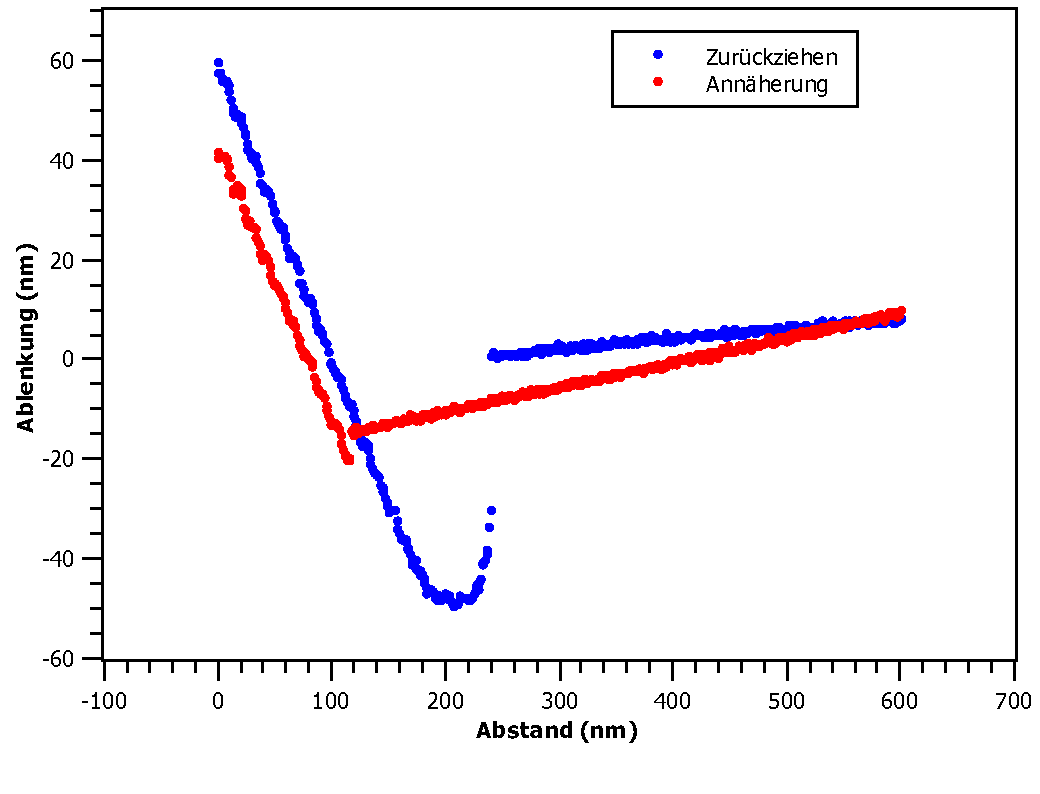
\includegraphics[width=.49\linewidth]{images/DVD/DS2}}
			\subcaptionbox{snap-off $s=\SI{42.4}{nm}$  \label{fig_dvd_ds3}}{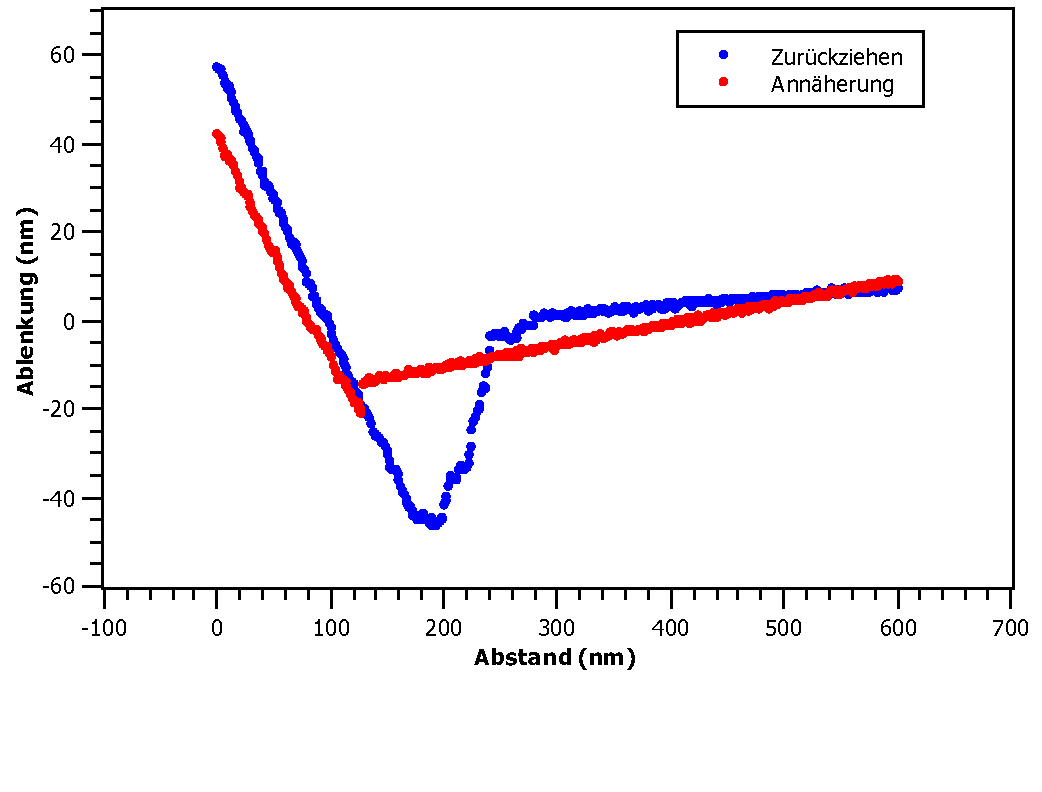
\includegraphics[width=.49\linewidth]{images/DVD/DS3}}
			\subcaptionbox{snap-off $s=\SI{44.2}{nm}$  \label{fig_dvd_ds4}}{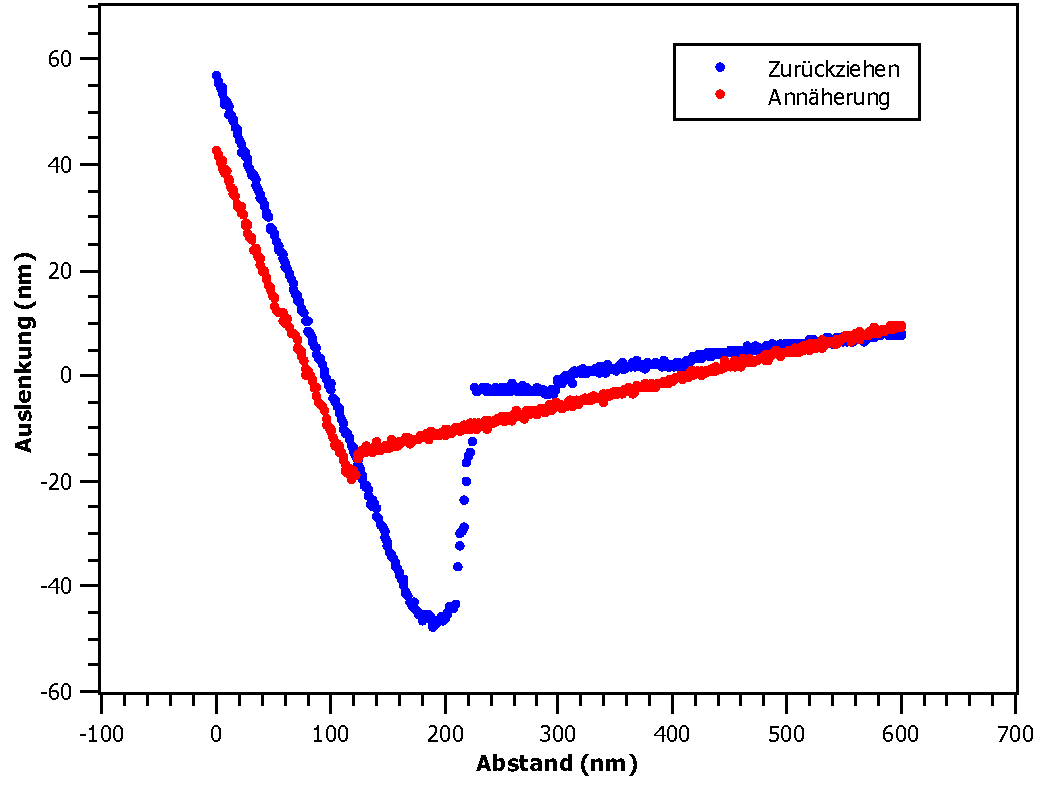
\includegraphics[width=.49\linewidth]{images/DVD/DS4}}
			\subcaptionbox{snap-off $s=\SI{39.8}{nm}$
			\label{fig_dvd_ds5}}{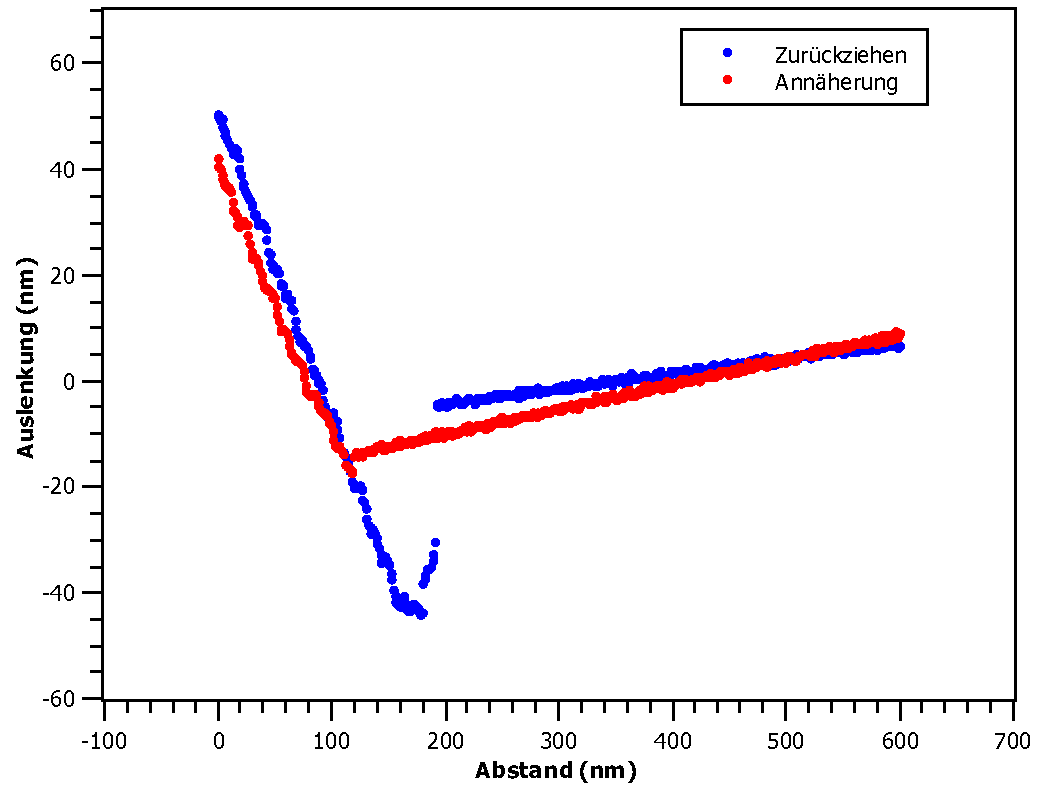
\includegraphics[width=.49\linewidth]{images/DVD/DS5}}
			\caption{Kraft-Abstands-Spektroskopie der Probe 1 auf einem der Maxima. Gemittelter snap-off $s=\SI{44.5}{nm}$.} % Pit oder Peak?
			\label{fig_dvd_ds}
\end{figure}
\begin{figure}[H]
			\centering
			\subcaptionbox{ snap-off $s=\SI{46.2}{nm}$\label{fig_cd_ds1}}{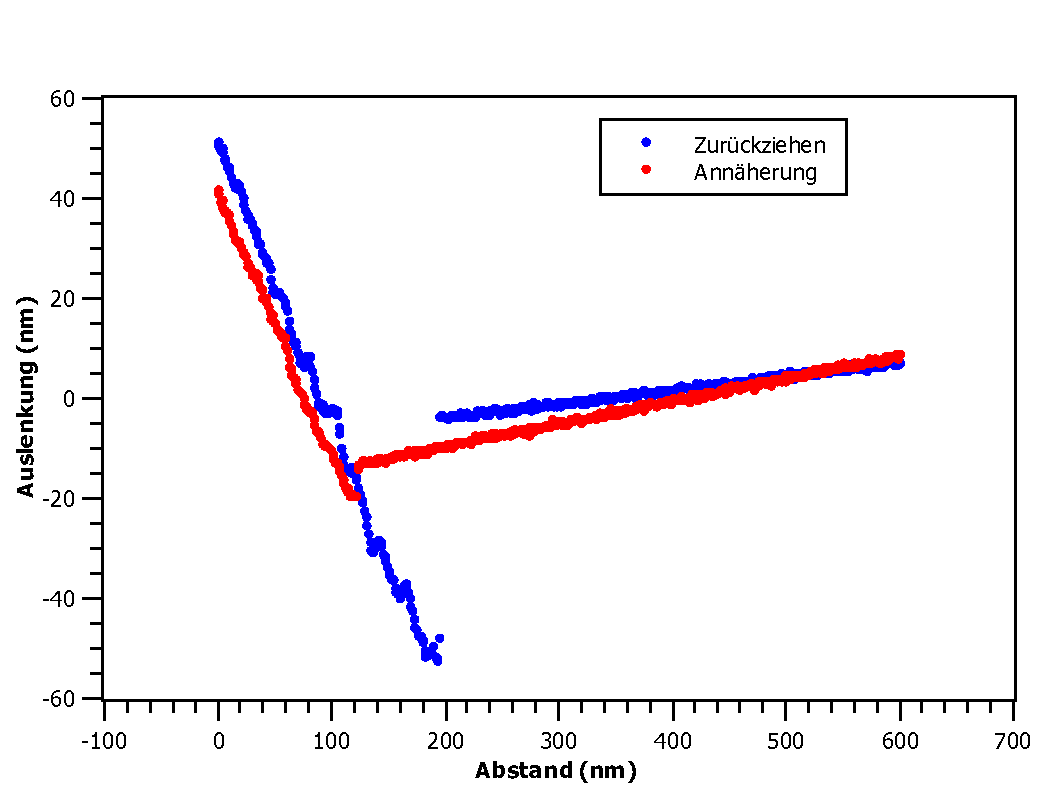
\includegraphics[width=.49\linewidth]{images/CD/DS1}}
			\subcaptionbox{ snap-off $s=\SI{50.2}{nm}$\label{fig_cd_ds2}}{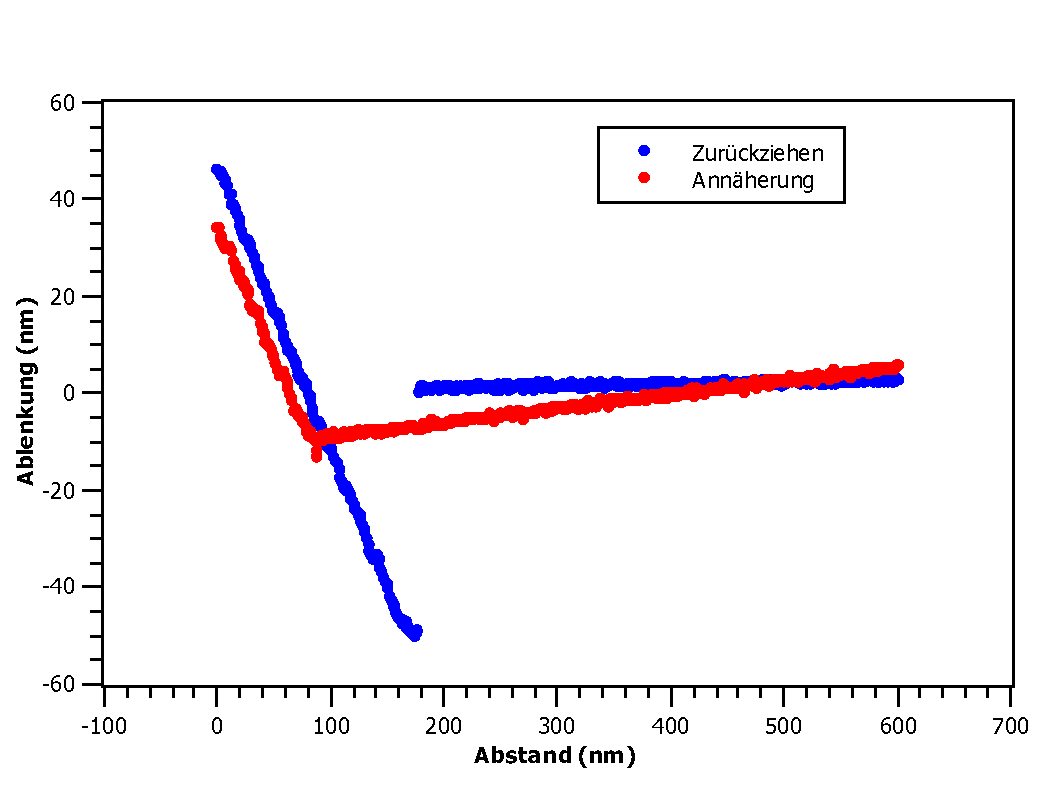
\includegraphics[width=.49\linewidth]{images/CD/DS2}}
			\subcaptionbox{ snap-off $s=\SI{53.5}{nm}$\label{fig_cd_ds3}}{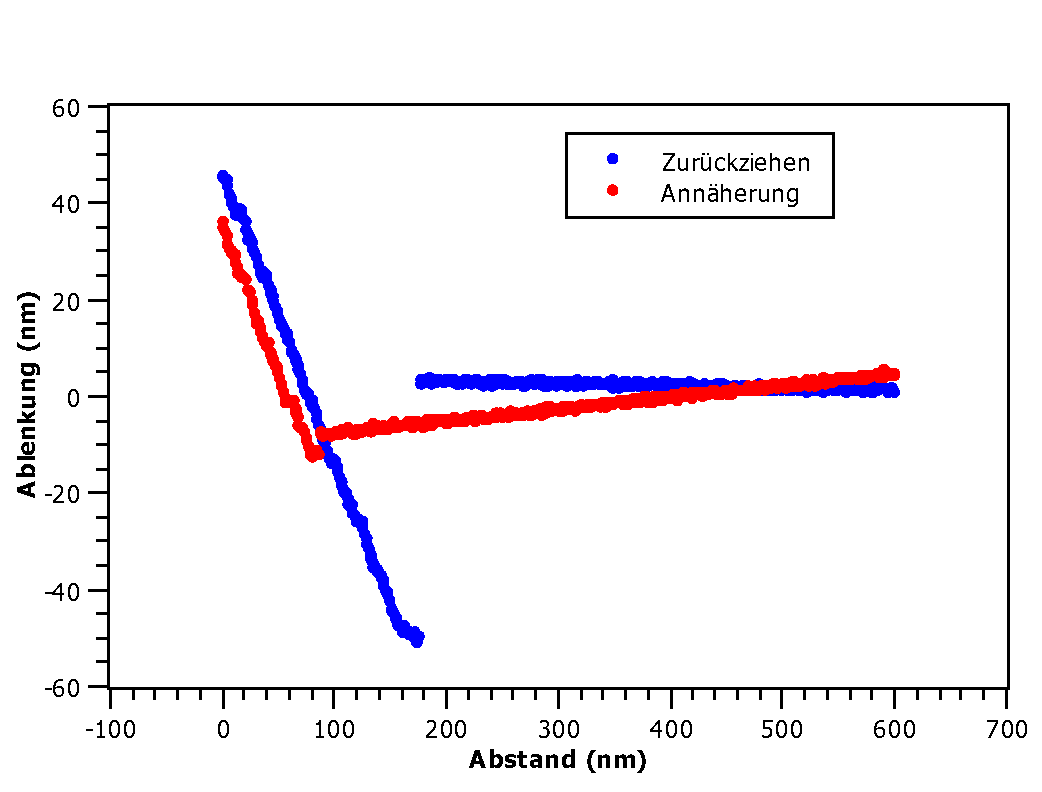
\includegraphics[width=.49\linewidth]{images/CD/DS3}}
			\subcaptionbox{ snap-off $s=\SI{53.7}{nm}$\label{fig_cd_ds4}}{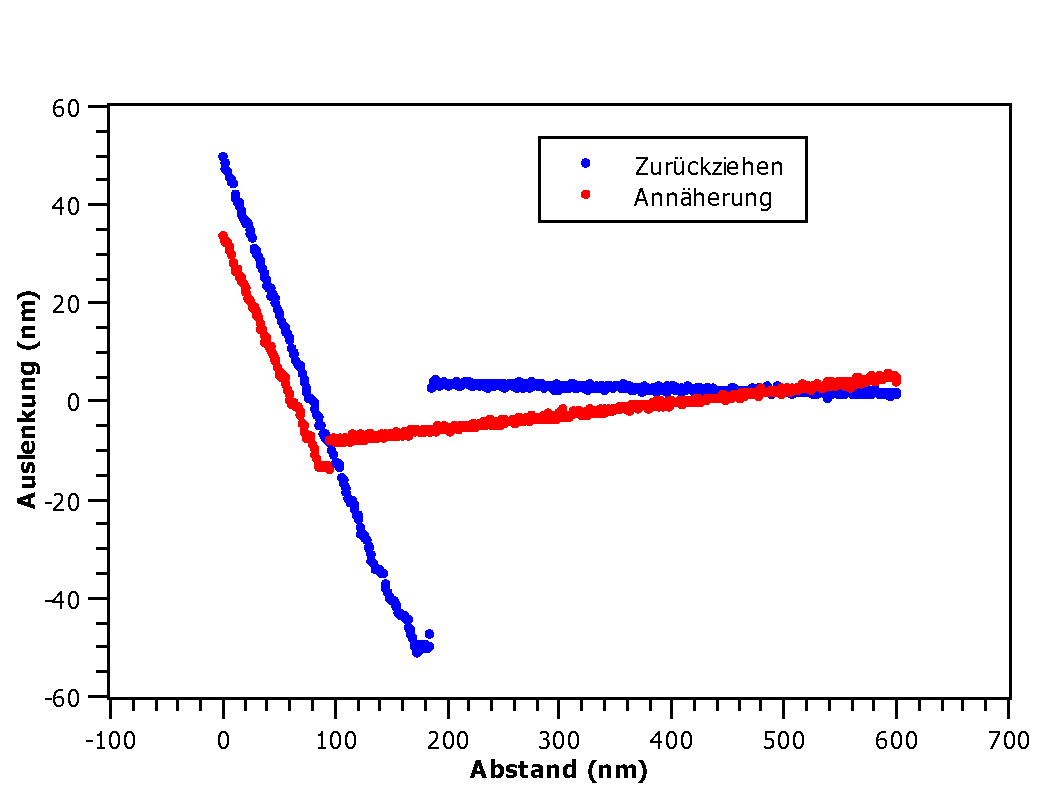
\includegraphics[width=.49\linewidth]{images/CD/DS4}}
			\subcaptionbox{ snap-off $s=\SI{47.8}{nm}$
			\label{fig_cd_ds5}}{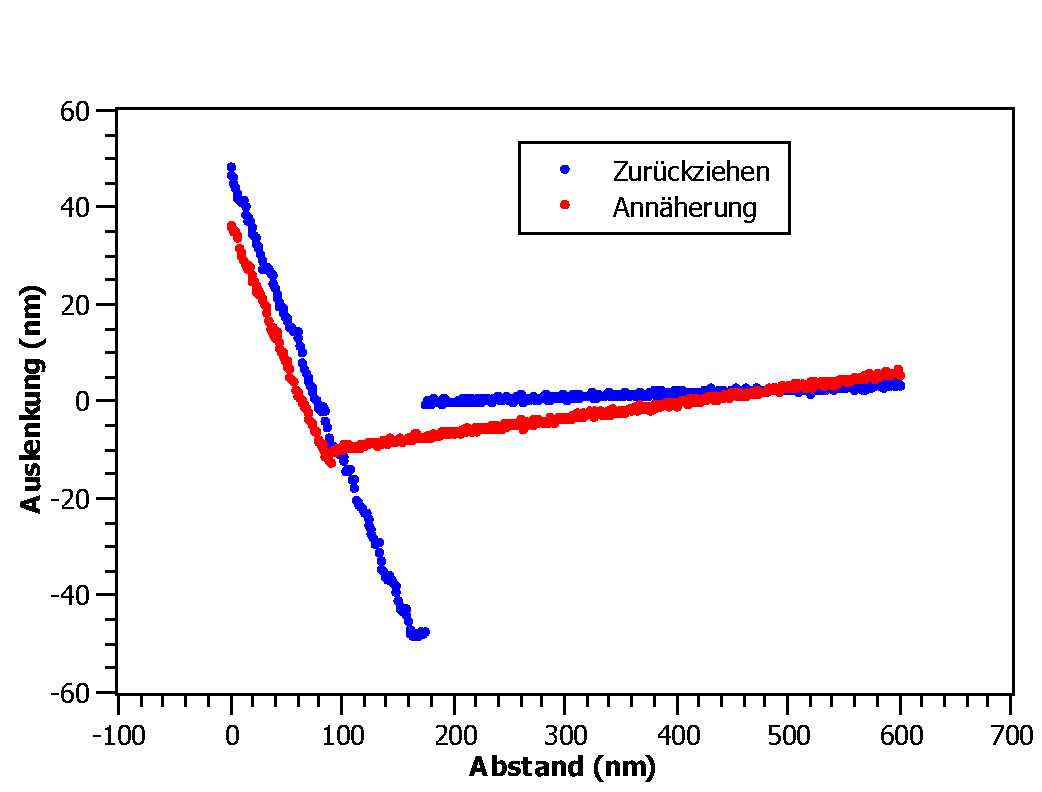
\includegraphics[width=.49\linewidth]{images/CD/DS5}}
			\caption{Kraft-Abstands-Spektroskopie der Probe 2 auf einem der Maxima. Gemittelter snap-off $s=\SI{50.6}{nm}$.} % Pit oder Peak?
			\label{fig_cd_ds}
\end{figure}

\begin{figure}[H]
			\centering
			\subcaptionbox{ snap-off $s=\SI{33.3}{nm}$\label{fig_br_ds1}}{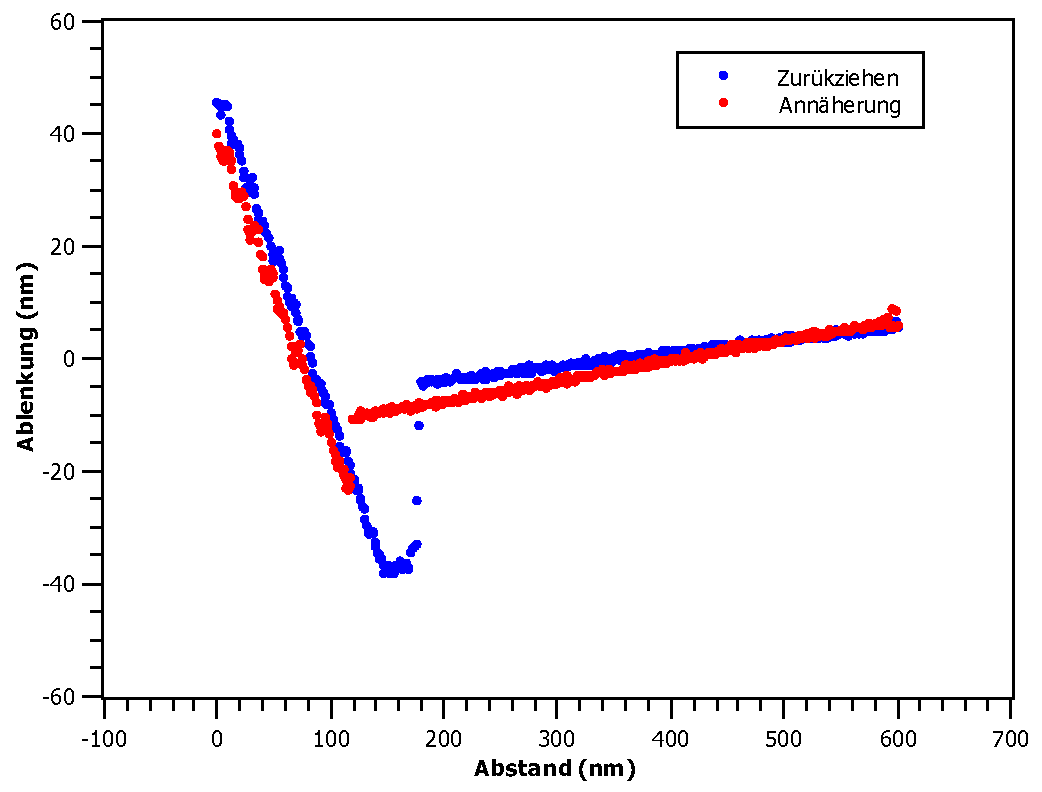
\includegraphics[width=.49\linewidth]{images/BR/DS1}}
			\subcaptionbox{ snap-off $s=\SI{35.6}{nm}$\label{fig_br_ds2}}{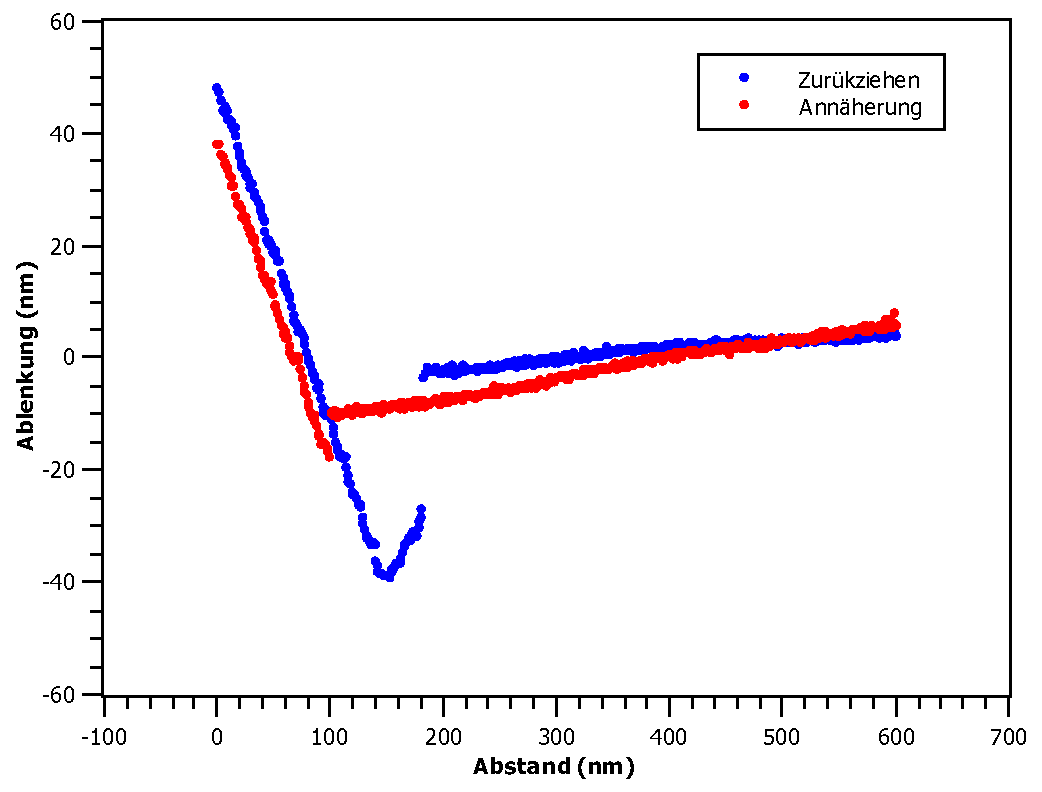
\includegraphics[width=.49\linewidth]{images/BR/DS2}}
			\subcaptionbox{ snap-off $s=\SI{35.3}{nm}$\label{fig_br_ds3}}{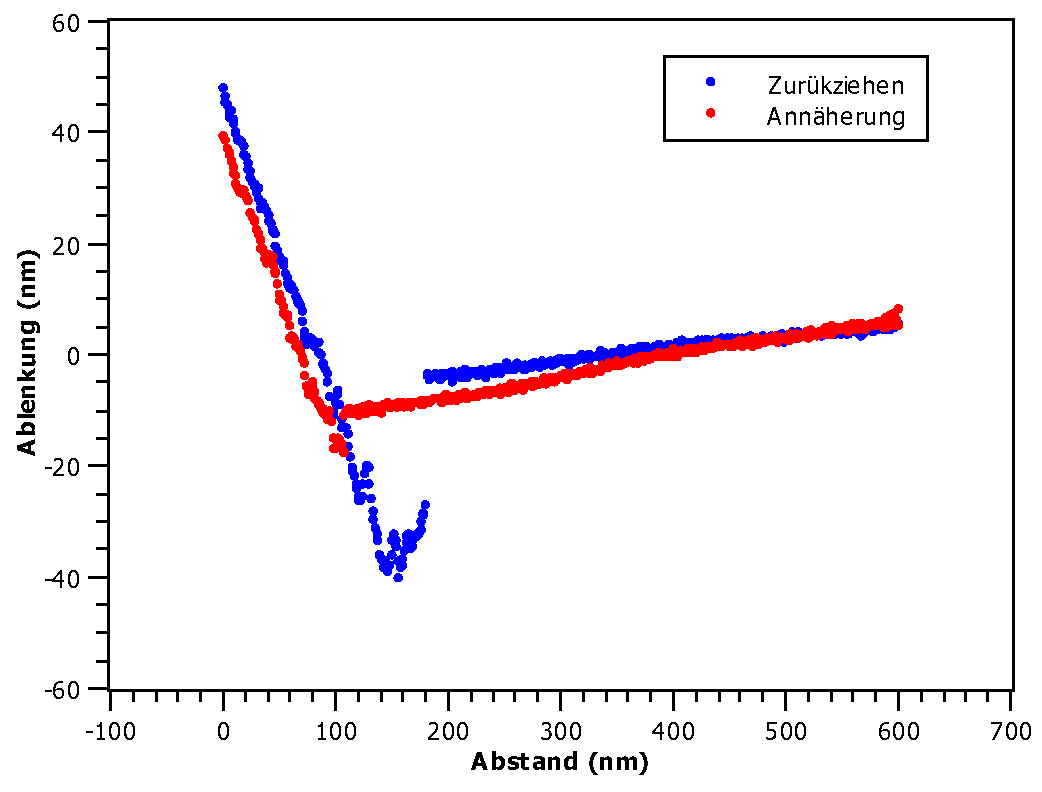
\includegraphics[width=.49\linewidth]{images/BR/DS3}}
			\subcaptionbox{ snap-off $s=\SI{35.7}{nm}$\label{fig_br_ds4}}{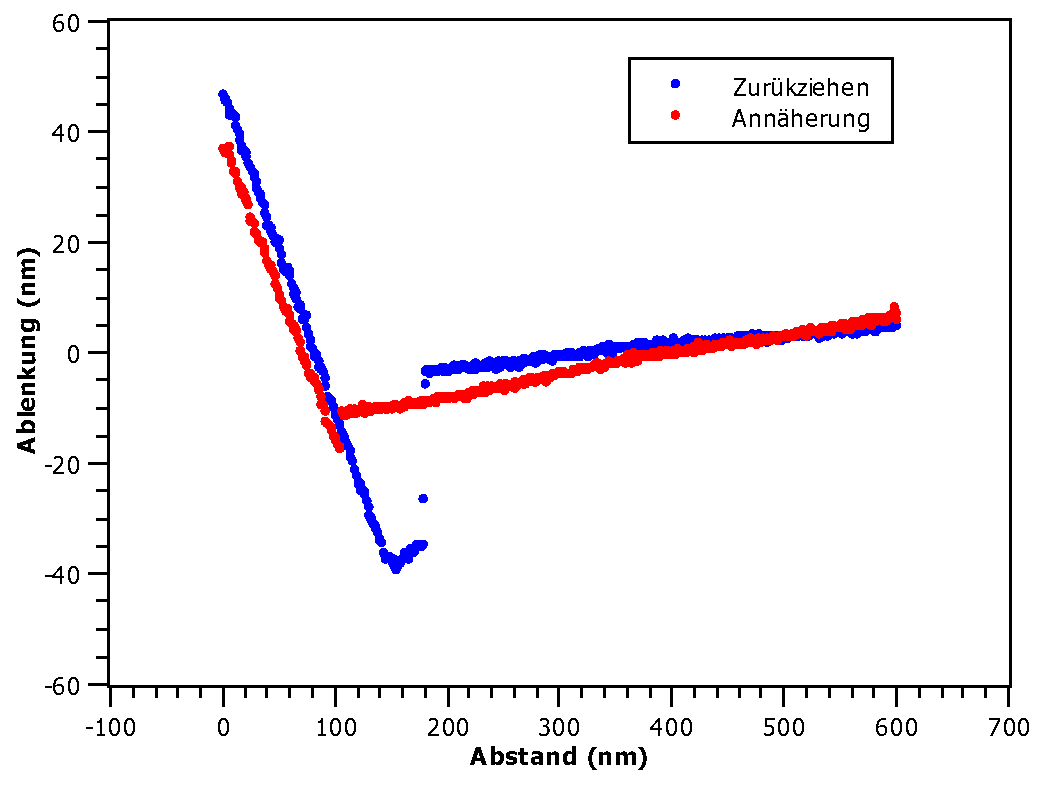
\includegraphics[width=.49\linewidth]{images/BR/DS4}}
			\subcaptionbox{ snap-off $s=\SI{36.4}{nm}$
			\label{fig_br_ds5}}{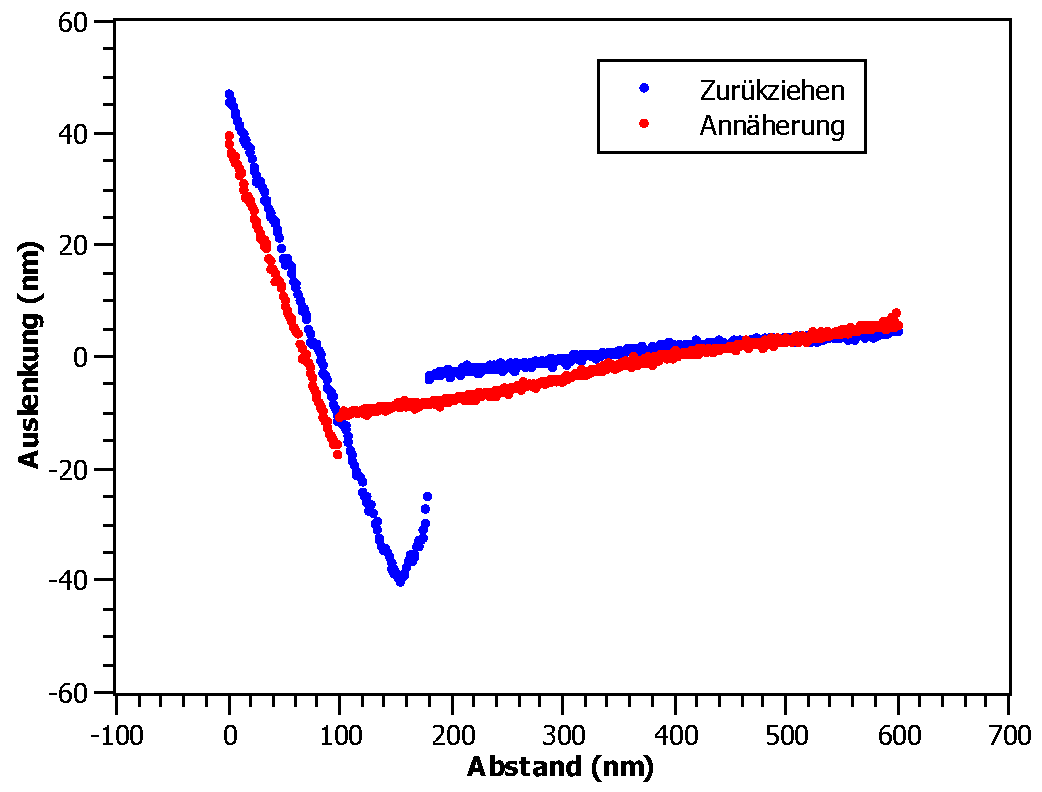
\includegraphics[width=.49\linewidth]{images/BR/DS5}}
			\caption{Kraft-Abstands-Spektroskopie der Probe 3 in einem der Minima. Gemittelter snap-off $s=\SI{35.3}{nm}$.} % Pit oder Peak?
			\label{fig_br_ds}
\end{figure}
%TODO Check Picture quality

\end{document}
